\phantomsection
\addcontentsline{toc}{chapter}{\textbf{Introduction en français}}
\onehalfspacing
\chapter*{Introduction en français }

L'humanité se trouve dans une ère écologique critique, où les seuils écologiques du système terrestre ont été franchis. La notion de "frontières planétaires" \citep{rockstrom2009safe,steffen_2015_planetary} illustre la façon dont l'anthroposphère, les effets des activités humaines à l'échelle de la planète, est devenue une composante fonctionnelle supplémentaire et est capable de modifier le système terrestre \citep{richardson_earth_2023} aux côtés de la géopshère (flux d'énergie et matériaux non vivants de la Terre et de l'atmosphère) et de la biosphère (tous les organismes vivants/écosystèmes). Le cadre des « limites planétaires » identifie les limites de l'impact de l'anthroposphère sur le système terrestre qui peuvent sauvegarder l'état interglaciaire de la Terre - le seul où la civilisation est connue - en identifiant un "espace opérationnel sûr". Parmi ces neuf limites, \cite{richardson_earth_2023} estime que six ont été franchies, menaçant la stabilité et la résilience du système terrestre. 

\begin{figure}[h]
	\centering
	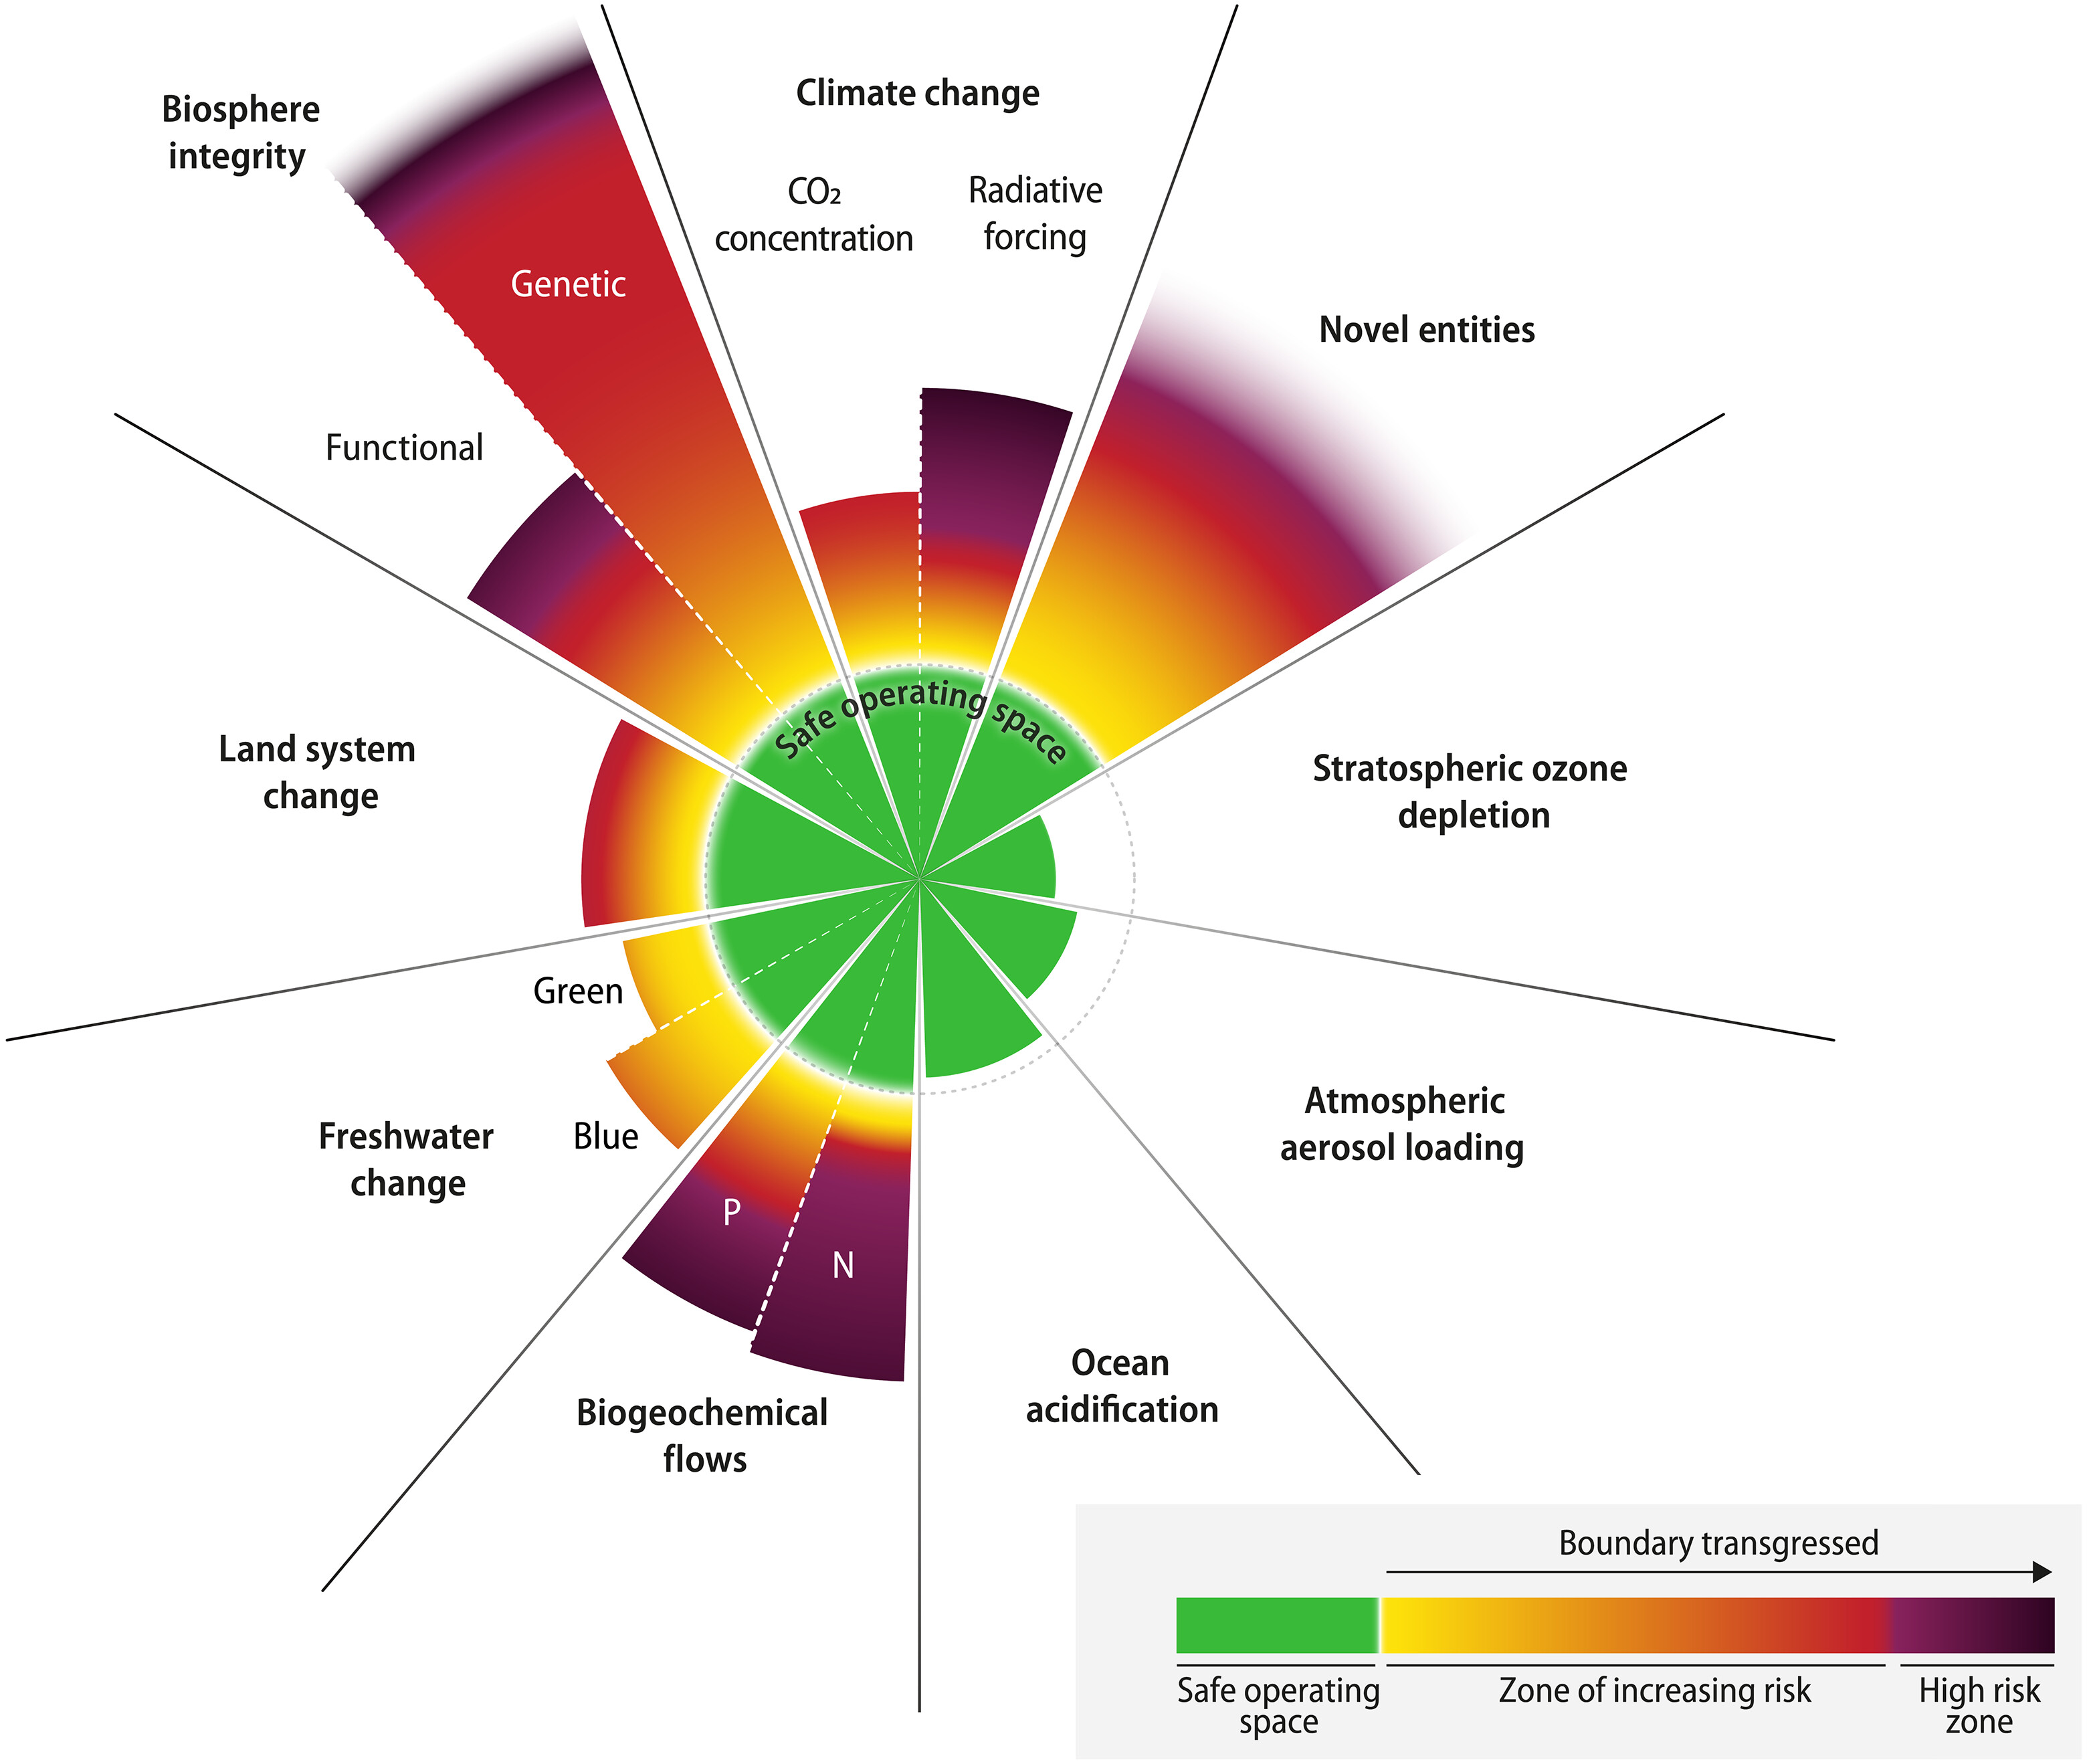
\includegraphics[width= .7\textwidth]{figures/intro/planetary_bounds.jpg}
	\caption{État actuel des variables de contrôle pour les neuf limites planétaires, à partir de \cite{richardson_earth_2023}}
\end{figure}

Parmi ces limites planétaires, l'intégrité de la biosphère a progressivement suscité un intérêt particulier, de même que son interaction avec d'autres limites, telles que le changement climatique, ou des entités nouvelles (par exemple, les polluants organiques synthétiques, les matières radioactives, la pollution microplastique...). Créé en 2012, le Groupe interdisciplinaire sur la biodiversité et les services écosystémiques (IPBES) a tiré la sonnette d'alarme sur l'état de la « Nature » à l'échelle mondiale. Son président, Sir Robert Watson, l'a clairement exprimé : « \footnote{Voir le \href{https://www.ipbes.net/news/Media-Release-Global-Assessment}{adresse du communiqué de presse du rapport 2019}} :
\begin{displayquote}
« \textit{Les preuves accablantes du \cite{ipbes_2022_6417333} Évaluation mondiale, provenant d'un large éventail de domaines de connaissances, présentent un tableau inquiétant [...]. La santé des écosystèmes dont nous et d'autres espèces dépendons se détériore plus rapidement que jamais. Nous sommes en train d'éroder les fondements de nos économies, de nos moyens de subsistance, de notre sécurité alimentaire, de notre santé et de notre qualité de vie dans le monde entier} »
\n-{displayquote}

La « nature » est un concept central dans le cadre de l'IPBES \citep{ipbes_2022_6417333} :

\begin{displayquote}
\citep{ipbes_2022_6417333} : \begin{displayquote} \textit{La nature (également définie comme la nature vivante) [est] le monde non humain, y compris les caractéristiques coproduites, avec un accent particulier sur les organismes vivants, leur diversité, leurs interactions entre eux et avec leur environnement abiotique. Dans le cadre des sciences naturelles, la nature comprend, par exemple, toutes les dimensions de la biodiversité, les espèces, les génotypes, les populations, les écosystèmes, la biosphère, le fonctionnement des écosystèmes, les communautés, les biomes, les systèmes de maintien de la vie sur Terre et leurs processus écologiques, évolutifs et biogéochimiques associés, ainsi que la diversité bioculturelle. Dans le cadre de l'économie, il comprend des catégories telles que les ressources naturelles biotiques, le capital naturel et les actifs naturels. Dans le contexte plus large des sciences sociales et humaines et des sciences environnementales interdisciplinaires, il est fait référence à des catégories telles que le patrimoine naturel, l'environnement vivant ou le non-humain. Dans le contexte d'autres systèmes de connaissance, il comprend des catégories telles que "Terre mère" [...], "Pachammama" [...]}.
\hspace*{\fill} \small{\cite{ipbes_2022_6417333}, p.14, voir aussi \cite{DIAZ20151}}
\small{cite{ipbes_2022_6417333}

La nature, telle qu'elle est définie dans cette approche, est un objet très vaste et complexe. Elle se définit à travers des différences ontologiques et épistémiques (vivant et non-vivant), différents types d'interactions, à diverses échelles (génotypes v. écosystèmes), à différents types de processus (biologiques v. écologiques), et à travers différents champs d'investigation (sciences naturelles v. sciences sociales). Dans cette thèse, j'étudie plus spécifiquement la "biodiversité", qui se concentre sur la variabilité des organismes vivants. Bien qu'il s'agisse d'un concept ambigu, la biodiversité tend à mettre l'accent sur les organismes vivants, en relation avec leur environnement matériel, biotique et abiotique (par opposition à l'étude de l'environnement non vivant) et sur son rôle essentiel parmi les autres composantes du système terrestre.

Le rapport \cite{ipbes_2022_6417333} documente les changements drastiques que subit la biosphère et examine ces changements dans une optique \textit{anthropocentrique}, c'est-à-dire en médiatisant les changements susmentionnés par les contributions multiples et diverses que la nature et la biodiversité apportent à l'homme. Il souligne l'impact de leur perturbation sur la vie humaine et met en évidence le rôle des facteurs anthropogéniques (c'est-à-dire d'origine humaine) dans la perturbation de la nature et de la biodiversité. 
 
Le présent rapport fixe différents objectifs à la recherche scientifique. Le premier objectif est d'expliquer les mécanismes de rétroaction : comment les moyens de subsistance de l'homme influencent-ils la biodiversité ? En réponse, comment la biodiversité influe-t-elle sur les moyens de subsistance de l'homme ? Cet objectif implique, d'une part, de comprendre les causes et de mesurer les facteurs anthropiques directs et indirects de changement dans la nature et la biodiversité et, d'autre part, de comprendre les canaux et les échelles par lesquels la nature et la biodiversité contribuent aux moyens de subsistance de l'homme, ainsi que de mesurer ces contributions. Par conséquent, l'étude de la disparition de la nature et des possibilités d'y remédier nécessite une perspective intégrée, qui associe les sciences naturelles aux sciences sociales, par le biais de cadres tels que les systèmes socio-écologiques \citep{Ostrom2009} ou l'économie environnementale et écologique \citep{daly_ecological_2007}. 
\\
Le deuxième objectif est de fournir un cadre pour évaluer l'opportunité, la faisabilité et les moyens de mise en œuvre des voies collectives qui permettraient de remédier à la crise à laquelle la nature est confrontée. D'une certaine manière, il s'agit de concevoir et de mettre en œuvre des voies politiques vers des avenirs durables, c'est-à-dire de trouver des voies ou des méthodes d'action définies choisies parmi des alternatives, aux niveaux individuel, collectif ou gouvernemental, pour parvenir à des états futurs du monde qui restent dans un espace de fonctionnement sûr en ce qui concerne les limites planétaires \citep{rockstrom2009safe,steffen_2015_planetary}.

Dans cette thèse, j'aborde ces deux objectifs en utilisant un cadre issu de l'économie et de l'écologie. Une première version des questions de recherche que cette thèse vise à résoudre est la suivante : 

\begin{enumerate}
\item Quelles sont les relations de rétroaction entre la biodiversité et les facteurs anthropogéniques de son déclin ? 
\item Quels sont les mécanismes sous-jacents auxquels les politiques doivent s'attaquer pour remédier à ce déclin ?
\item Comment les approches économiques et écologiques intégrées peuvent-elles être utilisées et affinées pour analyser, informer et concevoir des politiques publiques? 
\end{enumerate}

Afin d'affiner ces questions, je commence par définir le concept de biodiversité, à travers ses évaluations en sciences naturelles et sociales, et je souligne les tendances actuelles de sa disparition.

\phantomsection
\addcontentsline{toc}{section}{Emergence et définition de la biodiversité comme concept écologique}
\subsection*{Emergence et définition de la biodiversité comme concept écologique }


La biodiversité est apparue en tant que concept dans les années 1980, parallèlement à l'émergence de la « biologie de la conservation », une branche de la biologie qui s'intéresse à la protection de la « diversité biologique » \citep{soule_what_1985}, en réponse à l'accélération de la disparition des espèces. La position morale de la biologie de la conservation est que les espèces doivent être protégées pour elles-mêmes \citep{soule_conservation_1986}, elles ont une valeur intrinsèque. 
Le concept de biodiversité s'inscrit donc dans un jugement éthique et un appel à l'action. Dans le sillage de la conférence des Nations unies sur l'environnement et le développement qui s'est tenue à Rio en 1992, la \href{https://www.cbd.int/}{Convention sur la diversité biologique} s'est imposée comme un traité international visant à sauvegarder la biodiversité. Ce faisant, elle a fourni une définition internationalement reconnue :

\begin{displayquote}
« \textit{ La « Diversité biologique » désigne la variabilité des organismes vivants de toute origine y compris, entre autres, les écosystèmes terrestres, marins et autres écosystèmes aquatiques et les complexes écologiques dont ils font partie ; cela comprend la diversité au sein des espèces et entre espèces ainsi que celle des écosystèmes.}\\
\hspace*{\fill} \small{\href{https://www.cbd.int/convention/articles/default.shtml?a=cbd-02}{Article 2 of the Convention on Biological Diversity}}\footnote{Traduit par l'auteur}
\end{displayquote}

Cette définition met en évidence un élément clé de différenciation par rapport à d'autres parties de la nature, à savoir la nature vivante des objets étudiés. Par rapport aux facteurs abiotiques, la diversité biologique se caractérise par une croissance, une reproduction et un métabolisme intrinsèques (au niveau de l'individu et de la population), ainsi que par une évolution (au niveau de la génétique et de l'espèce). En outre, ces taux de changement dans le temps sont commensurables avec l'expérience humaine, et la plupart des processus (par exemple, la reproduction, l'effondrement ou la reconstitution des populations, l'évolution génétique) peuvent être observés au cours d'une vie humaine, par opposition à l'échelle temporelle géologique. 

Comme le soulignent \cite{VanDyke2008} et \cite{mouysset_diversity_2023}, la définition de la biodiversité est difficile, car elle recouvre des dimensions éthiques, conceptuelles et de mesure. La biodiversité peut être considérée comme « une qualité intrinsèque et sans valeur des systèmes naturels qui devrait être préservée pour elle-même » \citep{VanDyke2008, mouysset_diversity_2023}, mais elle se réfère également à des caractéristiques mesurables.
%
Cette définition implique différentes échelles d'un point de vue hiérarchique, au niveau génétique, au niveau de l'espèce, de la communauté et de l'écosystème (défini comme l'interaction des communautés et de leur environnement abiotique). Ces niveaux impliquent différentes formes de mesure, notamment la distribution des gènes, l'abondance des espèces (par exemple le nombre d'individus dans une population, à un moment et à un endroit donnés), la richesse des espèces (par exemple le nombre d'espèces différentes, à un moment et à un endroit donnés) au sein des communautés, entre les communautés et à des échelles plus grandes (par exemple les diversités alpha, bêta et gamma), ainsi que les variations des facteurs abiotiques qui forment les écosystèmes, tels que la température, l'humidité, la qualité de l'eau, la qualité du sol, etc. 
Elle comprend également différents types de diversité : la diversité structurelle (par exemple, les couches de la canopée dans les forêts, le sex-ratio dans les populations animales), la diversité de composition (la variété et l'abondance des espèces au sein d'une communauté) et la diversité fonctionnelle (la variété des processus environnementaux réalisés par les organismes vivants dans une zone donnée, par exemple la séquestration du carbone, le cycle des nutriments ou la dispersion des graines, voir \cite{loreau_biodiversity_2002}).

\begin{figure}
	\centering
	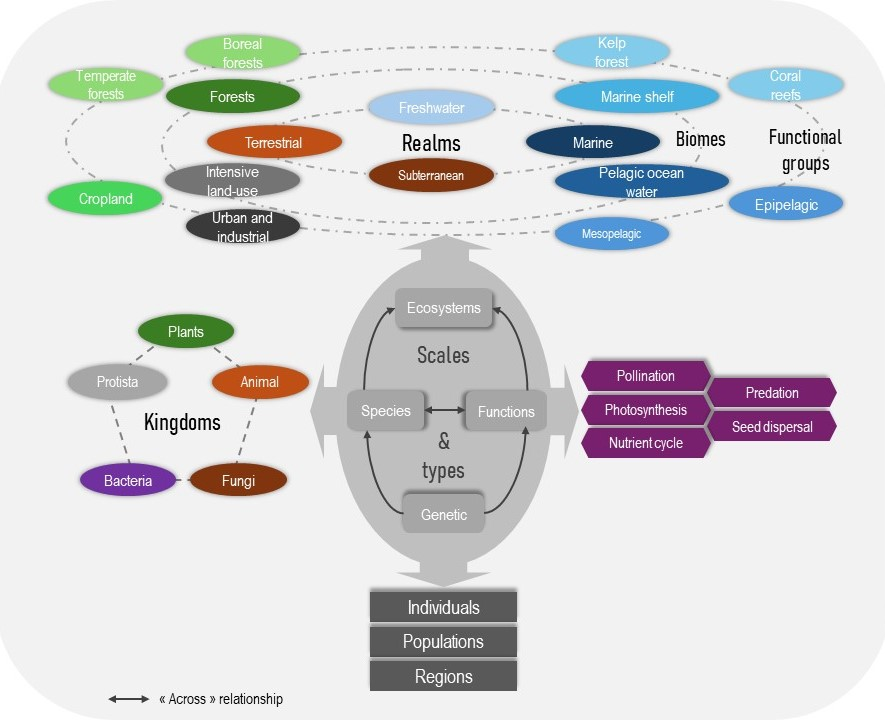
\includegraphics[width =.8\textwidth]{figures/intro/biodiv_illustration.jpg}
	\caption{ La biodiversité : un concept multiforme à travers échelles et types}
	\label{fig:intro_biod}
\end{figure}

\cite{mouysset_diversity_2023} souligne la difficulté d'articuler la définition avec les niveaux communs de l'analyse scientifique, par exemple génétique, taxonomique et écosystémique, car le niveau de biodiversité peut se situer entre les deux : « Les populations peuvent être considérées d'un point de vue génétique et taxonomique, ou les communautés qui se situent entre les niveaux taxonomique et écosystémique. En outre, la diversité structurelle et compositionnelle pouvant être considérée comme la source de la diversité fonctionnelle, il peut être difficile de travailler avec les différentes classes de diversité en raison de leur colinéarité. 

Les multiples dimensions de la biodiversité mettent en évidence plusieurs de ses caractéristiques essentielles. Tout d'abord, il est impossible de mesurer la biodiversité à l'aide d'un seul indicateur. L'étude de la biodiversité nécessite de multiples indicateurs pour évaluer de manière intégrée l'évolution de la biodiversité, à toutes les échelles et pour tous les types de diversité. L'émergence du concept répond à un désir de protéger la biodiversité pour son propre bien, mais aussi pour celui de l'humanité. 

\clearpage

\phantomsection
\addcontentsline{toc}{section}{Les Contributions de la Nature  aux Populations : logiques de conservation de la biodiversité}
\subsection*{Les Contributions de la Nature aux Populations : logiques de conservation de la biodiversité}

D'abord descriptives, les fonctions des écosystèmes ont été de plus en plus considérées d'un point de vue humain à partir des années 1970 \citep{hueting1969functions, schumacher1973small}, évoluant vers le concept de services écosystémiques \citep{ehrlich1981extinction} pour illustrer les conséquences de la perte de biodiversité \citep{gomez_history_2010}. Cette évolution a marqué le passage d'une valeur intrinsèque à une valeur anthropocentrique (c'est-à-dire donnée par l'homme) \citep{mouysset_diversity_2023}, reconnaissant les valeurs instrumentales et relationnelles de la biodiversité - servir les objectifs de l'homme et favoriser des relations significatives. Progressivement, la biodiversité a dû être protégée pour son rôle dans le maintien de la vie humaine.

Le concept a fait son chemin dans la recherche universitaire, et lorsque \cite{Costanza1997} a quantifié la valeur du capital naturel et des services écosystémiques à un montant stupéfiant de 33 trillions \$USD, soit environ 30\% du PIB mondial de 2020, le concept est entré dans l'arène politique. En 2005, l'Évaluation des écosystèmes pour le millénaire (Millenium Ecosystem Assessment \citep{MEA2005}) a placé les services écosystémiques au centre de l'agenda politique : elle a souligné une valeur anthropocentrique des services écosystémiques, mais a établi une dépendance des sociétés humaines aux services écosystémiques, et plus loin, au fonctionnement de l'écosystème. À cet égard, l'Évaluation des écosystèmes pour le millénaire (Millenium Ecosystem Assessment \cite{MEA2005}) a marqué un tournant dans la sauvegarde de la biodiversité par le biais d'un paradigme de \textit{soutenabilité forte} (voir encadré 1), et a déclenché l'opérationnalisation du concept dans les politiques à grande échelle (ce que je développerai plus loin). Le cadre des services écosystémiques a été divisé en 4 catégories, liées au type spécifique de services contribuant au « bien-être humain “ : les services de soutien (par exemple, les services permettant à d'autres services écosystémiques d'être présents, y compris le cycle des nutriments et la production primaire) et les services de régulation ("avantages obtenus par la régulation des processus écosystémiques", par exemple la pollinisation, la décomposition des déchets, la gestion de l'eau, etc. ) ; les services culturels ("les avantages non matériels que les gens tirent des écosystèmes par l'enrichissement spirituel, le développement cognitif") et les services d'approvisionnement ("tous les produits tirés des écosystèmes",\cite{MEA2005}, p.54 )

\begin{figure}[h]
	\centering
	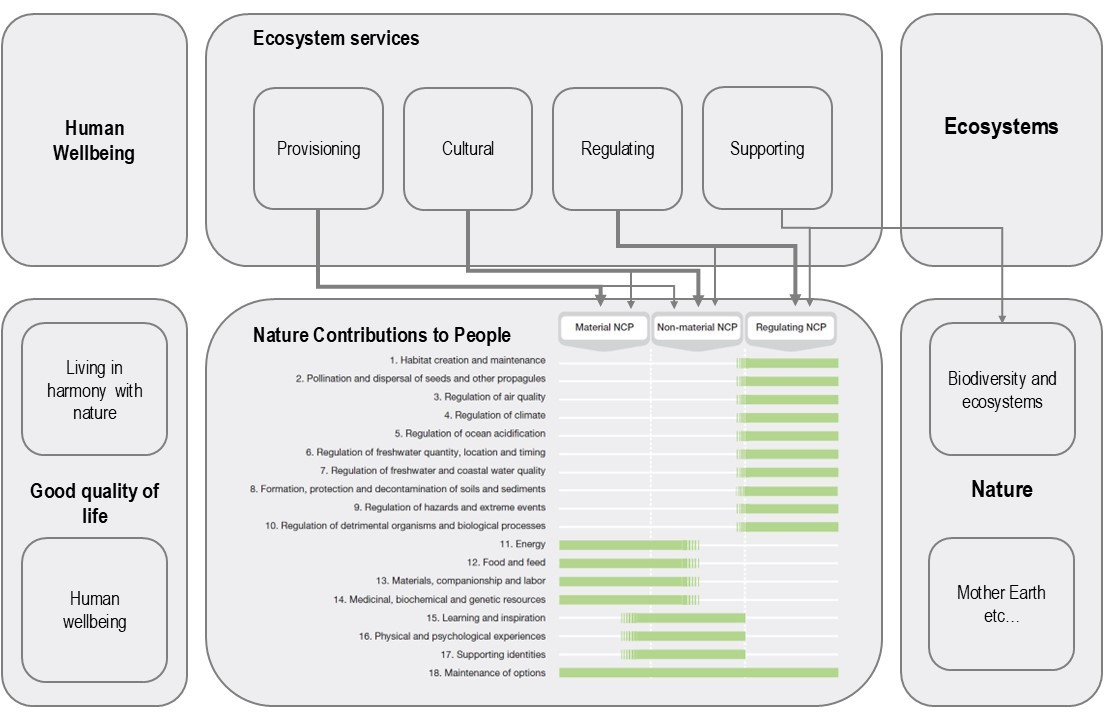
\includegraphics[width = \textwidth]{figures/intro/NCPs2.jpg}
	\caption{Description des 18 Contributions de la Nature aux Populations et du lien entre le cadre des CNP \citep{ipbes_2022_6417333} et le cadre des services écosystémiques \citep{millennium2005ecosystems}}}
	\subcaption*{Adapté depuis \cite{diaz_2018} et \cite{ipbes_2022_6417333}}
\end{figure}

Récemment, la plateforme IPBES est passée à un nouveau cadre conceptuel mettant en évidence les contributions de la nature aux populations (CNP) \citep{DIAZ20151}, définies comme « toutes les contributions, positives et négatives, de la nature vivante [...] à la qualité de vie des populations \citep{diaz_2018} ». Ce cadre sous-tend trois types de contributions aux personnes : les contributions matérielles aux personnes (flux de la nature vers les personnes généralement consommés pour « faire fonctionner une société ou une entreprise » (IPBES, p.16), les contributions non matérielles (par exemple, les effets de la nature sur « les aspects subjectifs et psychologiques qui sous-tendent la qualité de vie des populations ») et les contributions régulatrices (par exemple, « les aspects fonctionnels et structurels des organismes et des écosystèmes qui modifient les conditions environnementales vécues par les personnes et/ou régulent la génération de contributions matérielles et non matérielles »). Ce cadre met en évidence le fait que les contributions de la nature à l'homme peuvent être positives ou négatives et dépendent de la définition spatiale et temporelle de la contribution, puisqu'une entité donnée peut être à la fois la source de contributions positives et négatives : par exemple, les forêts favorisent l'habitat, mais risquent également de mettre en danger les personnes en cas d'incendies de forêt. En outre, elle offre une vision plus globale que les services écosystémiques, car elle englobe des perspectives allant de la biodiversité en tant que capital naturel utilisé dans une fonction de production écologique (voir \cite{polasky_integrating_2009} pour une revue), ainsi que des perspectives où la biodiversité a une agence et est liée par des obligations de soins réciproques envers les humains \citep{descola}. 

Une correspondance à multiples facettes entre les différentes composantes et dimensions de la biodiversité et ses contributions à l'homme est à la base des moyens de subsistance de l'homme. Le déclin mondial de la biodiversité menace les CNP.

\clearpage
\begin{tcolorbox}[breakable, 
colback=verylightgray, 
colframe=gray!75!black, 
title= {Box 1 - Soutenabilité Faible et Forte},
%code={\singlespacing},
fontupper=\small]
\par % This \par ensures spacing before the text starts
\justifying % Start justified text

En 1987, la publication du rapport Brundtland \citep{brundtland} a donné une définition large du développement durable : 

\begin{displayquote}
\textit{"Par essence, le développement durable est un processus de changement dans lequel l'exploitation des
ressources, la direction des investissements, l'orientation du développement technologique et les changements institutionnels sont tous en harmonie et améliorent le potentiel actuel et futur de satisfaction des besoins et des aspirations de l'humanité"}\\
\hspace*{\fill}\small{\cite{brundtland}, p.43}
\end{displayquote}

La mise en œuvre du développement durable est restée une question ouverte. En économie, une « perspective de durabilité faible », inaugurée par les travaux de \cite{hartwick_intergenerational_1977} et \cite{solow_intergenerational_1986} sur les ressources épuisables, suggérait que « le maintien d'un stock de capital non décroissant, qui pourrait être mis en pratique en investissant dans le capital manufacturé toutes les rentes dérivées de l'exploitation des ressources naturelles non renouvelables » \citep{gomez_history_2010} était suffisant pour maintenir la consommation au fil du temps. Dans cette approche, le capital naturel pouvait être intégralement remplacé par le capital humain. D'autre part, l'approche de la « durabilité forte » prône la complémentarité, plutôt que la substituabilité, des ressources naturelles \citep{costanza_daly}, reconnaissant ainsi la dépendance des humains à l'égard des écosystèmes.

\end{tcolorbox}

\N-phantomsection
\addcontentsline{toc}{section}{Déclin de la biodiversité : tendances et facteurs}
\subsection*{Déclin de la biodiversité : tendances et facteurs}

Les mesures de la biodiversité diminuent à toutes les échelles d'analyse. Les conditions structurelles des écosystèmes, la composition des communautés écologiques et des populations d'espèces ont connu des changements spectaculaires.
La part des habitats sauvages protégés et inchangés s'est effondrée sur terre et en mer \citep{watson_2016_catastrophic, jones_2018_location} pour atteindre 23\% et 12\% de l'espace, respectivement. Au niveau des communautés, la part de la biodiversité initialement présente tombe en dessous de 90 \% dans tous les biomes, \citep{Hill311787} et les communautés locales deviennent de plus en plus semblables \citep{mckinney_1999_biotic}, sous l'effet de l'augmentation de l'étendue des espèces invasives animales et végétales non aliens, en hausse de 13 \% par décennie \citep{seebens_no_2017}. Au niveau des espèces, à ce jour, la richesse des espèces mondiales est menacée par une extinction massive, car le taux mondial d'extinction des espèces est au moins dix fois plus élevé que le taux moyen des 10 derniers millions d'années et s'accélère \citep{barnosky_has_2011, ceballos_accelerated_2015}. En moyenne, 25 \% des espèces sont actuellement menacées d'extinction à l'échelle mondiale dans un large éventail d'espèces végétales et animales, sur terre et en mer \citep{IUCN_redlist_2024}. Utilisation de méthodes basées sur l'habitat La liste rouge de l'UICN utilise des comptes détaillés pour les espèces, dans une approche ascendante, afin d'analyser le risque d'extinction des espèces. Une approche descendante, qui s'appuie sur l'évolution de l'habitat disponible et la relation espèce-zone, utilise les changements dans l'utilisation des terres pour prévoir l'extinction des espèces de manière plus globale. \citep{Diamond1972BiogeographicKE}}, \cite{Hoskins309377} constatent que des centaines de milliers d'espèces végétales et animales sont menacées et rembourseront la \textit{dette d'extinction} causée par les changements anthropogéniques de leurs habitats : seulement 92.1\% des espèces de vertébrés terrestres, 91,6\% des invertébrés terrestres et 90,7\% des plantes terrestres disposent d'un habitat suffisant pour subsister. Ces résultats suggèrent qu'environ un demi-million d'espèces animales et végétales terrestres - dont plus de 3 000 vertébrés et plus de 40 000 plantes - sont condamnées à s'éteindre, à moins que leurs habitats ne s'améliorent à temps pour l'empêcher \citep{ipbes_2022_6417333}.

Les facteurs de déclin de la biodiversité sont d'origine anthropique. Ils peuvent être classés en deux catégories : les facteurs \textit{directs}, qui découlent directement des actions humaines, comme le changement d'utilisation des terres, le changement climatique anthropique, la surexploitation, et les facteurs \textit{indirects}, qui peuvent être considérés comme la cause première des facteurs directs, comme les changements dans les systèmes de valeurs qui sous-tendent les utilisations de la nature (\cite{ipbes_2022_6417333} p. 55), la démographie (urbanisation et migration), la technologie, l'économie (transitions sectorielles, expansion du commerce) et la gouvernance (y compris les systèmes de risque pour l'accès aux ressources). ), la démographie (urbanisation et migration), la technologie, l'économie (transitions sectorielles, expansion du commerce) et la gouvernance (y compris les systèmes de droits d'accès aux ressources).

Une synthèse des sciences naturelles réalisée par \cite{ipbes_2022_6417333} souligne le rôle des principaux facteurs à l'échelle mondiale et dans tous les domaines (voir figure \ref{fig:intro_impacts}).
Il montre que l'utilisation des terres et des mers, le repositionnement vers la perte, la fragmentation, la perte d'habitat sont sans aucun doute les principaux moteurs du déclin de la biodiversité terrestre. Les effets de la fragmentation sur la biodiversité sont très controversés. D'un point de vue théorique, des modèles ont été développés pour étudier l'évolution des populations et des communautés dans l'espace et le temps, par exemple les modèles de métapopulation et de métacommunauté. Les connaissances théoriques soulignent que la fragmentation de l'habitat augmente le risque d'extinction et réduit la probabilité de colonisation, ce qui se traduit par une baisse de la survie et de la diversité \citep{adler_persistence_1994,hill_habitat_1999, thompson_loss_2017}. À l'échelle communautaire, l'augmentation de la diversité entre les communautés (par exemple, la diversité bêta) peut résulter des différentes exigences des espèces en matière de ressources et de la plus grande étendue spatiale, qui englobe donc une plus grande hétérogénéité environnementale, résultant de la fragmentation \citep{lasky_reserve_2013, chisholm_species_2018}. Toutefois, ces effets s'atténuent à mesure que la perte d'habitat diminue.  
Au niveau empirique, l'effet de la fragmentation est très discuté. Selon \cite{fahrig_ecological_2017}, il n'existe aucune preuve empirique qu'un groupe de petites parcelles d'habitat a généralement une valeur écologique inférieure à celle de grandes parcelles de la même superficie totale. Des éléments montrent toutefois que la fragmentation ne réduit pas la connectivité des habitats, car la connectivité fonctionnelle est améliorée (par exemple, les espèces sont en contact avec un plus grand nombre de parcelles de ressources différentes, ce qui améliore le fonctionnement global des écosystèmes). Le débat entre \cite{fletcher_is_2018} et \cite{fahrig_habitat_2019} porte sur les critiques fondées sur la capacité des modèles statistiques à englober l'effet de la fragmentation en cas de perte d'habitat \citep{ruffell_accounting_2016}. En outre, il reflète la difficulté de l'écologie du paysage, car différents mécanismes à travers les échelles, par exemple la parcelle, le paysage et la région d'étude, et des mesures, telles que la taille de la parcelle, l'isolement de la parcelle (par exemple la distance entre les parcelles) et la distance au bord de la parcelle (par exemple la distance au bord à l'intérieur de la parcelle) interagissent avec des interactions non linéaires possibles.}
%
L'exploitation directe de la faune et de la flore sauvages et la dégradation de l'habitat de la faune sont responsables de 30\% des impacts sur la biodiversité. L'exploitation directe de la faune, de la flore sauvage et des arbres représente 23 \% des impacts. Le changement climatique, qui se traduit par des modifications des conditions biogéographiques et des changements d'habitudes, a un impact sur les caractéristiques des espèces et l'évolution génétique, ce qui représente 14\% des impacts, et la pollution représente 14\% des impacts. Enfin, les espèces exotiques envahissantes représentent 11\%. Ces facteurs ont des impacts différents selon les écosystèmes et les biomes \citep{ipbes_2022_6417333}. 

\begin{figure}[h]
	\centering
	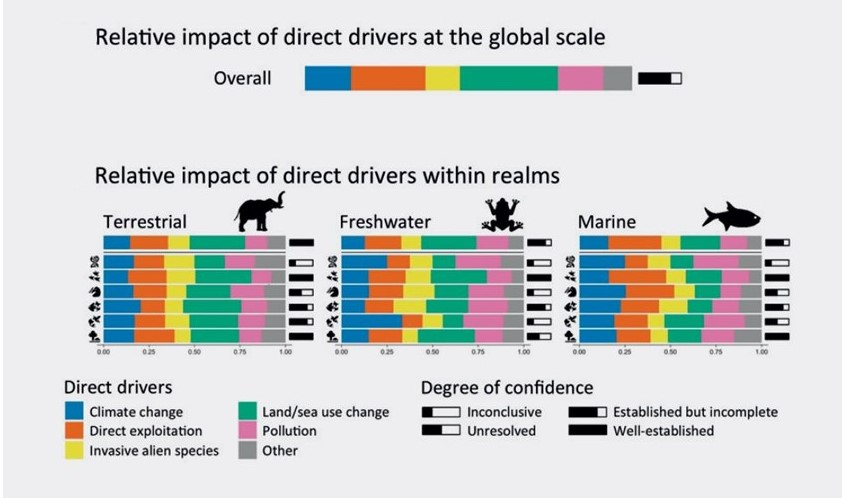
\includegraphics[width = .95 \textwidth]{figures/intro/intro_impactsfin.jpg}
	\caption{Aggregate and realms specific impacts of anthropogenic direct drivers of biodiversity decline adapted from \citep{ipbes_2022_6417333}}
	\label{fig:intro_impacts}
\end{figure}

Sur terre, le changement d'utilisation des terres est le facteur le plus important (30,5\%), sous l'effet de la déforestation et de l'agriculture, suivi de l'exploitation directe (21\%).     Les forêts tropicales et subtropicales sèches et humides abritent la plus grande diversité biologique. Par exemple, elles abritent les 10 hotspots qui comptent le plus grand nombre de vertébrés \citep{mittermeier_global_2011}. Dans ces forêts, la perte et la dégradation de l' habitat sont les principaux facteurs de réduction de l'abondance et de la richesse des espèces \citep{newbold_global_2014}. L 'exploitation forestière sélectivelégale et illégale détruit l' habitat \citep{hoare2022establishing, bousfield_2023_large} et est combinée à la chasse et au braconnage des espèces sauvages \citep{gallego_2020_combined}, générant entre 60 et 180 milliards \$ USD de revenus \citep{gfi_2017}\footnote{Le commerce illégal d' espèces sauvages représente entre 5 et 23 milliards \$USD, tandis que l'exploitation forestière illégale représente entre 52 et 157 milliards \$USD}. 

Pour les espèces marines, la surexploitation est le principal moteur (29\%) \citep{ipbes_2022_6417333}. Avec 90 millions de tonnes de captures (et 141 milliards de dollars américains) en 2020 \citep{fao_2022_state}, les stocks halieutiques se situant à des niveaux biologiquement durables ont diminué pour atteindre 64,6\% en 2019, contre 90\% en 1974 \footnote{ Dans ce calcul, tous les stocks halieutiques sont pris en compte de la même manière, indépendamment de leur abondance ou de leurs captures}, sous l'effet de la surpêche dans le Pacifique Sud-Est et dans les mers Méditerranée et Noire. Néanmoins, la pêche illicite, non déclarée et non réglementée (INN) constitue une menace pour les pêcheries.   Selon des estimations datant d 'il y a 15 ans \citep{agnew_estimating_2009} , elle représenterait entre 11 et 26 millions de tonnes de poisson pour une valeur de 10 à 23 milliards de dollars américains. 

En outre, le changement climatique anthropique entraîne des perturbations des écosystèmes sur terre \citep{burrell_anthropogenic_2020, conradi_reassessment_2024} et en mer \citep{gomes_marine_2024}, par le biais de changements dans divers canaux , y compris l' adéquation écologique et les perturbations du réseau trophique. Sur terre, par exemple, les forêts, lainages et broussailles méditerranéens, qui couvrent 4 millions de km², sont des zones d'une diversité exceptionnellement élevée \citep{Mooney2001, blondel_2010}, menacées par l' expansion urbaine et l'augmentation du risque d' incendie de forêt.     La fréquence et la gravité desincendies de forêt devraient augmenter avec le réchauffement climatique \citep{Dupuy2019ClimateCI}, entraînant d' importants coûts directs et indirects pour la société , notamment la destruction d ' infrastructures et des perturbations de l' activité économique \citep{wang_economic_2021}, les problèmes de santé liés à lafumée \citep{burke_wildfire_2023, heft-neal_behavior_2023}, la perturbation des caractéristiques structurelles des écosystèmes \citep{Ayars2023} et la menace pour la diversité biologique \citep{Wintle2020}.

\phantomsection
\addcontentsline{toc}{section}{Economic challenges of anthropogenic drivers}
\subsection*{Economic challenges of anthropogenic drivers}


La perte d'habitat et la surexploitation présentent des défis à la fois communs et différenciés.     Une cause commune identifiable est le coût d'opportunité élevé de la préservation de l'habitat ou de l'existence d'une espèce, en présence d'autres alternatives économiques pour la terre et le temps, ainsi que de contraintes financières. En outre, la perte d'habitat et la surexploitation partagent un aspect dynamique temporel, où les actions immédiates ont des conséquences durables, voire irréversibles.

La perte et la fragmentation de l'habitat dans les écosystèmes terrestres posent des problèmes spécifiques. Les forêts, par exemple, ont des usages multiples (ou PCN) pour différents agents : les bûcherons tirent profit du bois, les colons défrichent les terres pour l'agriculture, les randonneurs recherchent des paysages vierges et les défenseurs de l'environnement visent à rétablir les cycles naturels. Les forêts ont également une valeur spirituelle et culturelle, ce qui crée des conflits entre ces utilisations. Par exemple, la déforestation et l'urbanisation détruisent à la fois l'habitat et les terres sacrées, mais créent une valeur économique mesurée \citep{giglio_economics_2024}, tandis que la prévention des incendies de forêt peut endommager l'habitat des espèces sauvages \citep{bradshaw2018}. Les espèces peuvent également avoir des impacts mixtes ; les cerfs, par exemple, sont appréciés à faible densité mais causent des dommages à des densités plus élevées \citep{putman_identifying_2011}. 
Le changement climatique aggrave la perte d'habitat en modifiant la distribution des habitats et en augmentant les menaces telles que les incendies de forêt \citep{Dupuy2019ClimateCI,wasserman_climate_2023}.
    Une deuxième caractéristique essentielle pour mettre fin à la fragmentation des habitats est la prise en compte de l'ensemble des interdépendances, des retombées écologiques et des externalités économiques qui sous-tendent la dimension spatiale. La configuration de l'espace et le mouvement des espèces sont, au moins en partie, le résultat d'une décision économique.     Le maintien de la connectivité des habitats passe par l'identification des parcelles et des chemins à conserver ou à restaurer qui y contribuent le plus, sous forme de corridors, d'écoducs ou de tremplins \citep{Turner2005, Turner2011}. La valeur des parcelles et des chemins pour la connectivité est intrinsèquement liée à leur environnement : au même endroit géographique, une parcelle a une valeur différente pour l'habitat de la biodiversité si elle est connectée à d'autres, ou si elle est isolée (voir encadré 2). Lorsque les chemins échappent au contrôle de l'homme, les parcelles ont une importance différente en fonction de leur emplacement, et lorsque l'emplacement des parcelles est fixe, l'étendue des chemins et leur emplacement sont primordiaux.
\\
Troisièmement, lorsque des actions et des utilisations multiples structurent des éléments connectés des écosystèmes (par exemple, différentes étendues de terre ou différentes échelles de biodiversité), elles entraînent des retombées spatiales, c'est-à-dire des conséquences qui vont au-delà de leurs effets \textit{in situ}. Lorsque ces retombées ne sont pas prises en compte par les agents qui les génèrent, elles peuvent être appelées « externalités spatiales dynamiques » \citep{sanchirico_bioeconomics_1999, costello_optimal_2008, costello_private_2017}. Étant donné que l'arrêt de la perte et de la fragmentation des habitats implique la conservation de parcelles de terre, les parties voisines peuvent très bien bénéficier (ou souffrir) d'un plus grand nombre d'espèces sauvages et de (dis-)services écosystémiques sur leur propriété, au fil du temps. Comme les agents réagissent aux profils d'action des autres, ils adoptent un comportement \textit{stratégique}, à la fois dans l'espace et dans le temps. Ces externalités peuvent déclencher des problèmes spécifiques de « race to the bottom » \citep{costello_private_2017} : lorsque les parties voisines d'un décideur qui entreprend la conservation, ou la réduction des risques, ne parviennent pas à se rendre la pareille alors qu'elles bénéficient des retombées, un cercle vicieux de moindre action est déclenché. Inversement, lorsque les retombées écologiques sont positives, cela peut conduire tout le monde à utiliser une ressource à des niveaux non durables, même en présence de droits bien définis, en l'absence d'autres mécanismes \citep{janmaat_sharing_2005,kaffine_unitization_2010}. 
Par conséquent, la fragmentation de l'habitat et la surexploitation sont liées par la connectivité spatiale. 
\\
Quatrièmement, l'amélioration de la perte et de la fragmentation des habitats implique la coordination de nombreux acteurs en vue d'accroître la superficie et la connectivité des habitats, tout en tenant compte des coûts et des avantages associés, ainsi que des différents intérêts.
Dans certains cas, les contraintes financières, l'ampleur des coûts associés à l'augmentation de la connectivité des habitats et la difficulté de la coordination justifient une politique publique dans laquelle un planificateur central entreprend l'action \citep{Mouysset2012}. D'autre part, il existe des mécanismes permettant de décentraliser une planification spatiale efficace, qui peuvent être efficaces lorsque les coûts de coopération sont limités \citep{costello_private_2017, bareille_agglomeration_2023}. 

Pour mettre un terme à la surexploitation, il faut comprendre et traiter ses motivations. La surexploitation (ou le sous-contrôle, pour les parasites) résulte d'un déséquilibre entre l'appropriation et l'utilisation des contributions de la nature à l'homme (tant positives que négatives) et le niveau et la répartition socialement souhaitables de ces contributions, ainsi que du comportement stratégique non coordonné des agents. 	
La nature commune de la plupart des ressources naturelles \citep{Gordon1954, smith_models_1969} a longtemps été identifiée comme l'une des principales raisons de leur disparition : de nombreux événements ont montré une « course vers le bas », où l'absence de droits de propriété sûrs a accéléré la surexploitation et le déclin des populations. Cette question est depuis longtemps au centre de l'attention, et les mécanismes reposant sur l'attribution de droits de propriété ont fait l'objet d'études approfondies \citep{libecap_tragedy_2009, costello_partial_2015, isaksen_tragedy_2019}.


\begin{tcolorbox}[breakable, 
colback =verylightgray, 
colframe=gray!75!black,
title={Box 2 - Habitat Loss, Fragmentation and Connectivity},
%code={\singlespacing},
fontupper=\small]


\par % This \par ensures spacing before the text starts
\justifying % Start justified text

 
  La perte d' habitat correspond à la perte de zones présentant des conditions environnementales adéquates pour la survie et le développement des espèces.     À surface d'habitat constante, la fragmentation se traduit par une augmentation du nombre de parcelles et une diminution de la taille moyenne de chaque parcelle, comme le montre la figure \ref{fig:connectivity_intro}. \\

  La connectivité du paysage est définie par rapport à la fragmentation. Elle mesure "le degré auquel le paysage facilite ou entrave le mouvement entre les parcelles de ressources" \citep{taylor_connectivity_1993}. 

Elle recouvre une dimension \textit{structurelle}, qui décrit les arrangements physiques entre les parcelles, et une dimension \textit{fonctionnelle}, qui met l'accent sur la capacité et la réalisation des mouvements des individus à travers le paysage.

   Les mesures de connectivitéglobale tiennent compte du rôle des parcelles et des chemins différenciés. Dans le panneau D de la figure \ref{fig:connectivity_intro}, les parcelles encerclées jouent un rôle déterminant dans le maintien de la connectivité. Les parcelles d'habitat 1 et 2 ont le même nombre de parcelles connectées.     Cependant, la parcelle 1 maintient la connexion entre les parcelles d' habitat situées à l'est et à l'ouest du paysage et est reliée à des parcelles fortement connectées. Lasuppression des parcelles d' habitat 1 et 2 aurait des conséquences plus importantes sur l'habitat que la suppression d' autres parcelles de taille identique.     De même, la suppression du chemin en pointillé (en bas à gauche du panneau D) isolerait la parcelle 3, tandis que la suppression du chemin en pointillé ne laisserait pas la parcelle 4 isolée. Par conséquent, les chemins et les îlots ont des impacts différents sur la connectivité, en fonction des îlots et des chemins environnants.

\\% Adds some space before the image
\begin{center}
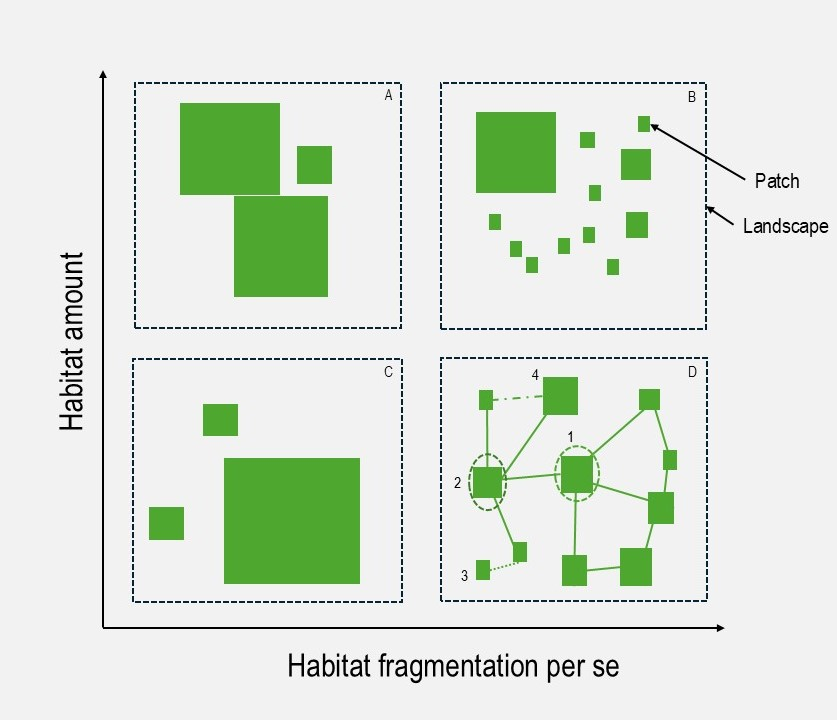
\includegraphics[width = .8\textwidth]{figures/intro/fragmentation.jpg}
\captionof{figure}{Illustration of the effects of habitat loss and fragmentation, adapted from \cite{fahrig_habitat_2019}, and of connectivity}
\label{fig:connectivity_intro}
\end{center}
\end{tcolorbox}

 
  Toutefois, si les droits de propriété peuvent être attribués, il est notoirement difficile de les faire respecter dans les régions où les fonctions régaliennes sont contestées:     \textit{de facto} les droits sont attribués et appliqués. Dans ce cas, la nature commune de la ressource peut ne pas être la principale préoccupation: les forces de concentration du marché local peuvent l'emporter sur les forces de surexploitation, même en présence d' une certaine forme d ' accès libre \citep{damania_economics_2007}. 

  Dans le monde entier, le braconnage et le commerce d' espèces sauvages sont généralement le fait de groupes criminels organisés et sont associés à différentes activités criminelles \citep{mozer_introduction_2023}.    Des marchésconcentrés tendent à émerger et à caractériser les marchés des espèces sauvages, car la concurrence est entravée par les groupes criminels organisés violents. Dans ce cas, la gestion des ressources est stratégique et répond aux caractéristiques du marché (structure de lademande, prix des intrants intermédiaires ) et aux caractéristiques écologiques (distribution des espèces, taux de croissance biologique, capacité de charge ). \footnote{La notion de \textit{capacité de charge} est utilisée depuis le milieu duXXème siècle par les écologistes des populations (pour un historique de la notion, voir \cite{sayre_carrying_2008}) pour décrire la taille maximale de la population d 'une espèce qu' un écosystème donné peut supporter à long terme.)

	À un extrême, une structure de marché monopolistique locale pour les produits de la faune sauvage peut émerger, en particulier dans le cas d' espèces endémiques (par exemple, indigènes et limitées à une zone).

Ils peuvent être les meilleurs amis des défenseurs de la nature\citep{solow_resources_1974, hannesson_note_1983}, en fonction des caractéristiques spécifiques du marché et des espèces, qui dépendent du contexte, car un monopoleur a intérêt à restreindre l' offre pour augmenter les prix, si les consommateurs ne réagissent pas trop (par exemple, en cas d' élasticité limitée de la demande ). Un large éventail de structures de marché \citep{damania_economics_2007, hannesson_effects_1985} collant à des situations réelles a été étudié.     Cependant, l ' ensemble des interactions entre l' endémisme d'une espèce, le pouvoir du marché local, le coût de l' effort et l'accès aux marchés de consommation finale nécessite une analyse plus approfondie afin de clarifier l ' impact de la structure du marché.

	  D 'autres facteurs de surexploitation peuvent être trouvés dans les bénéfices importants attendus (par rapport à d'autres activités économiques locales) que certaines ressources naturelles peuvent supporter, la plupart du temps en raison de leur rareté (par exemple, l ' absence de substitut économiquement viable), que ce soit aujourd'hui ou à l'avenir \citep{Kremer2000}.     Alors que les effets de la substitution de produits fabriqués par l'homme aux services écosystémiques perturbés commencent à faire l'objet d' études empiriques \citep{frank_economic_2024} et montrent à quel point les coûts peuvent être redoutables, l' effet de l' introduction de substituts aux produits de la faune sauvage braconnés illégalement peut être un exemple de forte substituabilité entre les actifs naturels et artificiels \citep{chen_economics_2017}. Comme des forces plus larges affectent la surexploitation, y compris la pauvreté, il est clair que le traitement de la surexploitation implique de généraliser la conclusion de l 'interaction d ' une seule espèce avec le cadre institutionnel, comment l ' avenir d'une espèce interagit avec la disponibilité des substituts, et comment la distribution des revenus provenant des récoltes durables peut favoriser une utilisation raisonnée de la ressource. 

	

	Un large éventail de politiques a été mis en œuvre à différents niveaux organisationnels, afin d' enrayer, conjointement ou séparément, les facteurs identifiés de déclin de la biodiversité sur terre et en mer, avec plus ou moins de succès. 



\phantomsection
\addcontentsline{toc}{section}{Biodiversity policies : from global to local}
\subsection*{Biodiversity policies : from global to local}
\par

  Les cadres politiques internationaux successifs ont cherché à enrayer la perte de biodiversité en s'attaquant à ses facteurs de manière globale.     En 2022, la 15e conférence de la Convention des Nations unies sur la diversité biologique a lancé le \href{https://www.cbd.int/doc/c/e6d3/cd1d/daf663719a03902a9b116c34/cop-15-l-25-fr. pdf}{Keunming Montreal Global Biodiversity Framework (GBF)}, remplaçant le Plan stratégique pour la biodiversité 2011-2020 et les Objectifs d' Aichi après avoir échoué à atteindre ses objectifs{footnote{Parmi les 20 Objectifs d' Aichi, aucun n'a été atteint au niveau mondial en 2020, et seulement 6 ont été partiellement atteints , y compris l ' identification et l'éradication des espèces envahissantes sur les îles, la désignation de 17\% des zones terrestres et des eaux intérieures et de 10\% des zones côtières et marines comme zones de conservation, la mise en œuvre d' instruments politiques et d'une stratégie et d'une planification nationales efficaces en matière de biodiversité, et l ' augmentation du financement de la protection de la biodiversité.   Lesraisons invoquées pour cet échec sont l ' absence d ' indicateurs clairs pour évaluer les objectifs, et l'absence d'obligation de rendre compte des progrès accomplis dans la réalisation des objectifs \citep{maron_setting_2021}}. Le GBF fixe quatre objectifs mondiaux pour 2050, avec 23 objectifs mesurables pour stopper la perte de biodiversité d' ici 2030. Ces objectifs comprennent le maintien de l' intégrité et de la connectivité des écosystèmes et la prévention des extinctions induites par l'homme(objectif A), l'utilisation durable de la biodiversité (objectif B), le partage équitable des avantages et des charges liés à la conservation (objectifs C et D)\footnote{Voir \href{https://www.cbd.int/doc/c/e6d3/cd1d/daf663719a03902a9b116c34/cop-15-l-25-fr.pdf}{Section G. Kunming-Objectifs globaux de Montréal pour 2050}}. \href{https://www.cbd.int/gbf/targets/5}{Les objectifs } comprennent la restauration de 30\% des écosystèmes dégradés, la conservation de 30\% des zones terrestres et marines et la garantie de l ' utilisation et de la gestion durables des espèces sauvages.
  
 
  D'autres traités internationaux , tels que la \href{https://cites.org/fra}{Convention sur le commerce international des espèces de faune et de flore sauvages menacées d'extinction (CITES)} établie en 1973, réglementent le commerce des espèces menacées d'extinction afin d' empêcher le commerce illégal des espèces sauvages \footnote{CITES compte 183 parties membres (pays), elle répertorie les espèces à travers des « annexes », avec différents degrés de protection des espèces et des restrictions limitant le commerce des espèces menacées d'extinction \\r}.

Annexe 1 : les espèces les plus menacées, menacées d ' extinction et dont le commerce international est interdit, sauf lorsque l' objectif des exportations n'est pas commercial.

Annexe 2 : espèces qui ne sont pas nécessairement menacées d' extinction à l'heure actuelle, mais qui pourraient le devenir si le commerce n'est pas étroitement contrôlé.

Annexe 3 : espèces inscrites à la demande d ' une Partie qui réglemente déjà le commerce de l 'espèce et qui a besoin de la coopération d' autres pays pour prévenir l' exploitation non durable ou illégale et promouvoir la survie de l' espèce.   Malgré sa portée, l'efficacité de la CITES est discutée. L'application au niveau local \citep{HEID2023102784} et les campagnes de réduction de la demande \citep{macfarlane_reducing_2022, moorhouse_demand_2024} sont essentielles, mais les interdictions commerciales peuvent parfois augmenter les prix et les incitations au braconnage \citep{hsiang_does_2016}. Dans certains cas, l ' agriculture de conservation a réussi à « inonder le marché » \citep{gentry_looking_2019, phelps_framework_2014, tensen_under_2016}. Les interventions du côté de l'offre ont parfois permis de réduire le braconnage et de reconstituer des populations sauvages - par exemple, la vigogne et le chat tacheté \citep{iucn_world_2000, sahley_biological_2007}- mais elles ont également échoué - par exemple, le chat tacheté et le chat sauvage - en raison de l 'absence d ' un système degestion des ressources naturelles. - mais elles ont également échoué - par exemple, le python vert, l'éléphant d' Afrique \citep{lyons_wildlife_2011, hsiang_does_2016}.   L'incertitude quant aux résultats des approches fondées sur le marché en matière de conservation a conduit à continuer de s'appuyer sur des interdictions et des contrôles du commerce qui sont souvent inefficaces pour réduire le braconnage.



Les politiques nationales et supranationales ont également joué un rôle clé.   Aux États-Unis, des politiques telles que \href{https://www.fs.usda.gov/Internet/FSE_DOCUMENTS/fseprd645666.pdf}{Wilderness Act of 1964} ont créé des zones protégées pour préserver les habitats. Dans le sillage du mouvement écologiste des années 1960 et 1970, des réglementations historiques visant à protéger les habitats naturels, telles que la \href{https://www.epa.gov/laws-regulations/summary-clean-water-act}{Clean Water Act de 1972} (garantissant que les eaux usées limitent la perturbation de l' habitat des espèces sauvages ), et visant spécifiquement la conservation des espèces avec la \href{https://www.fws.gov/sites/default/files/documents/endangered-species-act-accessible.pdf}{Endangered Species Act de 1973}. Lesrésultats de la loi sur les espèces menacées d'extinction font l'objet d'un débat. Si les impacts semblent globalement positifs sur le rétablissement des espèces, le budget consacré aux inscriptions est mince, et les coûts associés sont substantiels et concentrés sur les propriétaires privés alors que les bénéfices sont plus largement répartis \citep{brown_economics_1998, langpap_economics_2018}.

%

Des initiativeslocales, telles que \href{https://y2y.net/}{Yellowstone Yukon Conservation Initiative} (1993), relient des zones écologiques à travers les États-Unis et le Canada, en utilisant des programmes de conservation privés et l'élaboration de politiques locales . 

%

En Europe, le réseau Natura 2000 \footnote{Un système de zones protégées, établi en application de la directive Oiseaux (1976) et de la directive Habitats (1992) de l'Union européenne, et officiellement mis en place à partir du milieu des années 2000} a créé la plus grande zone de conservation au monde, couvrant 18 % des régions terrestres et 9 % des régions marines de l 'UE, à travers 28 000 sites. Dans les grandes lignes, elle délimite des zones de conservation d' intérêt écologique où le développement et les activités humaines sont limités. Son ambition était de prendre en compte l' échelle des processus de biodiversité plutôt que les frontières administratives pour développer un réseau interconnecté de zones de conservation. Les performances écologiques et économiques d' un tel réseau sont considérables, car elles génèrent des retombées spatiales à la fois en termes de performances économiques et écologiques \citep{cocco_relaxing_2023}.



Reconnaissant que l' habitat de la biodiversité peut être considéré comme un continuum entre des conditions inappropriées et appropriées, des mécanismes tels que les paiements pour services écosystémiques (PSE) sont mis à profit pour encourager la conservation sur les terres agricoles. En tenant compte des retombées écologiques de la diminution des retombées, les paiements pour les services écosystémiques assortis de primes d' agglomération, de sorte que les voisins bénéficient d'un avantage marginal supplémentaire lorsqu' un nouveau participant local met en œuvre des mesures de conservation, peuvent être efficaces \citep{parkhurst2002agglomeration, bareille_agglomeration_2023}. Dans l'ensemble, les conséquences spatiales des politiques décentralisées n' ont pas encore été pleinement intégrées dans l'élaboration des politiques.



Enfin, certaines politiques visent à atténuer les menaces que le changement climatique fait peser sur les écosystèmes et les espèces, en modifiant la connectivité des paysages. Dans les forêts méditerranéennes , où la biodiversité est exceptionnellement élevée mais où les incendies de forêt constituent une menace croissante \citep{Dupuy2019ClimateCI, wasserman_climate_2023}, les opérations de traitement des combustibles \footnote{L 'éclaircissement mécanique, les brûlages dirigés et , parfois, l 'exploitation forestière, ont été mis à profit pour réduire la charge de combustible dans les zones à risque et , théoriquement, pour diminuer la probabilité et la gravité des brûlures en cas d ' incendie de forêt. Dans de nombreuses régions, telles que les forêts de conifères de Californie \citep{Vaillant2009, Kalies2016, low_shaded_2023}, les forêts d' eucalyptus du sud-ouest de l'Australie \citep{burrows2013, boer_long-term_2009, Florec2020}, le sud de l 'Europe \citep{Fernandes2013}, il est prouvé que les traitements des combustibles peuvent atténuer l' intensité et la propagation des incendies de forêt.   Les agences de gestion des terres ont historiquement mis en œuvre ces politiques en Australie \citep{burrows2013}, en Europe et aux États-Unis (et devraient s ' intensifier, par exemple dans le cadre de l ' Infrastructure Investment and Jobs Act de 2021 aux États-Unis )} pour limiter l' occurrence et la gravité des incendies de forêt.   Les politiques publiques sont mises à profit pour faire face à l' augmentation des risques, à la limitation de l'assurabilité et aux menaces qui pèsent sur la biodiversité. Par exemple, l' assurabilité limitée des habitations situées dans l ' interface urbaine sauvage en Californie\footnote{Par exemple, \href{https://www.washingtonpost.com/climate-environment/2024/08/29/california-insurance-wildfires-allstate/}{200 000 propriétaires verront une augmentation de leur prime d' assurance } de 34,1\% en moyenne de la part de la compagnie d'assurance Allstate en novembre 2024. En 2023, le plan FAIR, conçu pour être l' assureur de dernier recours en Californie ( mandaté parl'État mais financé par le secteur privé ) a connu une augmentation de 38,3 % de son exposition totale. }}, ainsi que les dommages humains et non humains potentiels des incendies de forêt à l'échelle de l'économie\citep{wang_economic_2021, heft-neal_behavior_2023, Ayars2023 } les politiques de traitement des combustibles mandatées et gérées par l'État sont essentielles. Cependant, avec des budgets plus importants et un meilleur aménagement du territoire, ces politiques pourraient atteindre de meilleures performances en matière de réduction des risques tout en protégeant la biodiversité.

  Des mécanismes politiquesdécentralisés existent , tels que des mandats pour créer une zone tampon défendable autour des propriétés individuelles: en Californie, une zone défendable de 100 pieds autour des maisons est obligatoire dans les zones de responsabilité de l'État, et peut se traduire par des primes d' assurance réduites; en France, dans les régions dédiées, l' obligation de débroussaillement impose des opérations de contrôle des combustibles dans un rayon de 50 m pour « diminuer l ' intensité des incendies de forêt et limiter leur propagation ».

\footnote{Traduit par l ' auteur - \href{https://www.legifrance.gouv.fr/codes/article_lc/LEGIARTI000047809197}{Article L131-10} du Code Forestier} avec des amendes pouvant atteindre 5 000\$ euros en cas de non-respect.





Je me concentre sur l ' analyse de l ' interaction entre la biodiversité et les actions humaines, à travers les PCN qu' elle fournit et les moteurs anthropogéniques de son déclin. Étant donné que les politiques existantes ont eu des degrés de réussite variables dans l'arrêt du déclin de la biodiversité, un cadre pour l'élaboration des politiques est nécessaire. J'utilise un cadre issu de l'écologie et de l'économie pour analyser conjointement les causes de ce déclin et fournir des recommandations politiques. 


\phantomsection
\addcontentsline{toc}{section}{Biodiversity as an economic object}
\subsection*{Biodiversity as an economic object}

 
  La définition de l' économie s' est élargie avec de nouvelles méthodes et de nouveaux objets, mais elle se concentre principalement sur l'analyse du comportement humain aux niveaux individuel et collectif afin de gérer des ressources limitées à travers des alternatives \citep{mankiw_principles_2011, bade_foundations_2002, backhouse_retrospectives_2009}. Cela conduit à deux objectifs : comprendre et expliquer l ' état du monde ( approche positive) et déterminer les meilleures façons de gérer les ressources ( approche normative). L'économie fournit donc des outils pour analyser la perte de biodiversité et concevoir des politiques.



Cependant, l'application de l ' économie à la biodiversité est un défi.   Elle nécessite la mise en commun des valeurs, souvent par le biais d'une évaluation monétaire. Initialement , la biodiversité était évaluée pour ses produits (chasse, pêche, exploitation forestière) échangés aux prix du marché, en se concentrant sur les ressources dans un état spécifique - mortes. Cette approche ne prenait en compte qu' une partie de la « valeur d'usage » des espèces (dans le cadre du PCN, la « valeur d'usage » d'une espèce ). (dans le cadre des PCN, les PCN matériels associés à la nourriture et aux matériaux), sans tenir compte de leur valeur totale. Au fil du temps, la notion de « valeur d'usage » s'est élargie pour inclure les contributions directes et indirectes des espèces.   De nombreuses études ont utilisé des indicateurs de marché pour estimer le prix de la biodiversité \footnote{Par exemple, les méthodes hédoniques \citep{rosen_hedonic_1974} utilisent les variations des prix du marché pour des biens tels que l' immobilier liés aux caractéristiques environnementales, tandis que la méthode des coûts de voyage \citep{clawson_economics_1967, bhandari_willingness_2010} mesure les dépenses des consommateurs pour des expériences telles que l' observation de la faune et de la flore.}. Lorsque les indicateurs de marché échouent, par manque de données par exemple, des techniques d'évaluation non marchandes ont vu le jour \citep{carson_contingent_2012}, s'appuyant sur les préférences déclarées \footnote{Par exemple, à la suite de la marée noire de l'Exxon-Valdez en 1989, des enquêtes ont été mises au point pour estimer la valeur des ressources naturelles,     desétudes ont été mises au point pour estimer la valeur de la biodiversité affectée en demandant aux gens s'ils étaient prêts à payer pour la récupération \citep{carson_contingent_1992, arrow_report_1993, carson_contingent_2003}, bien que ces méthodes soient controversées \citep{Diamond94}} (par exemple, déclarées plutôt que déclarées). (par exemple, volonté de payer déclarée plutôt qu' observée ). 

 Avec le cadre des services écosystémiques, les techniques d'évaluation ont été mises à l'échelle pour capturer divers services \citep{Costanza1997}, y compris les efforts récents de modélisation globale \citep{giglio_economics_2024}. De multiples méthodes ont permis d'étendre l ' évaluation de la biodiversité à toutes les échelles, de la génétique aux habitats et aux fonctions \citep{bartkowski_capturing_2015}.

Récemment, les approches se sont détournées des mesures monétaires directes pour évaluer les effets des espèces sur des résultats tels que la santé \citep{frank_social_nodate,frank_economic_2024}. Un nombre important de recherches ont rejeté l' évaluation monétaire, se concentrant plutôt sur des mesures de la biodiversité à mettre en balance avec les résultats économiques \citep{Mouysset2011, Watzold2016a}.   Ces mesures permettent d' évaluer ou de planifier l'évolution de la biodiversité.


 
    Lagestion de la biodiversité implique d' équilibrer les alternatives tout en tenant compte de la spécificité des éléments vivants, des taux de régénération et d'extinction, ce qui nécessite de comprendre sa dynamique temporelle. L'économie fournit un cadre pour modéliser cette dynamique et évaluer l ' impact de différentes actions sur la biodiversité actuelle et future. Lesmodèles, en tant qu'« histoires structurées “ (\citep{GibbardVarian}), où la structure est ”la forme logique et mathématique d“ un ensemble de postulats » avec des « éléments d” interprétation » (\citep{GibbardVarian}), sont utilisés à diverses fins (voir l' encadré 3).

Parallèlement à l ' évolution des techniques d'évaluation monétaire, des \textit{modèlesbioéconomiques } ont été élaborés pour concevoir des politiques de gestion des ressources et de conservation de la biodiversité.

\begin{tcolorbox}[breakable, 
colback=verylightgray, 
colframe=gray!75!black, 
title= {Box 3 - What do models do? },
%code={\singlespacing},
fontupper=\small]


cite{varenne_epistemologie_2014} approfondit l ' approche « médiateur » et qualifie les modèles de facilitateurs, à travers de multiples dimensions. Une typologie non exhaustive des rôles que peuvent jouer les modèles comprend (i) un rôle pédagogique (faciliterla communication), (ii) un rôle prédictif (faciliter l' anticipation), (iii) un rôle heuristique (faciliter l ' explication d' un mécanisme avec quelques interactions simples), (iv) prescriptif (faciliter la réponse à un problème donné ) et (iv) intégratif (faciliter les échanges entre disciplines). 

\end{tcolorbox}

\phantomsection
\addcontentsline{toc}{section}{Bioeconomic modeling for the study and management of biodiversity}
\subsection*{Bioeconomic modeling for the study and management of biodiversity}

 
Les modèlesbioéconomiques sont des outils analytiques (par exemple, avec une formulation mathématique ) qui modélisent conjointement les rétroactions entre les composantes de la biodiversité dans les écosystèmes sauvages ou faiblement gérés et les activités économiques, à différents niveaux (par exemple, les niveaux micro, mezzo et macro). Ils combinent un modèle de décision issu de la théorie économique et la dynamique des éléments de la biodiversité issus de l'écologie. Les modèlesbioéconomiques \citep{Gordon1954, smith_models_1969, clark_profit_1973} sont nés des efforts conjoints des économistes et des écologistes pour gérer les ressources en tenant compte de la dynamique spécifique des éléments biotiques \citep{Parent_Mouysset_Missemer_Levrel_2024}\footnote{Comme le souligne \citep{Parent_Mouysset_Missemer_Levrel_2024}, la concavité de la « fonction de productionécologique », p. ex. des débarquements, résulte d'un effet de levier.     des débarquements, résultait de l 'application de la loi des rendements décroissants de l' effort humain.     Ce n'est qu' avec l' apport de Schaeffer que la concavité de la fonction de production écologique dans \cite{Gordon1954} a été fondée d'un point de vue écologique, à partir d'un argument de dynamique des populations (en utilisant une fonction de croissance logistique )} en tant que modèles véritablement interdisciplinaires (voir l' encadré 4). 



Historiquement, les premiers modèles bioéconomiques sont nés de l'écologie des populations et de l'analyse économique statique, pour étudier la gestion des pêcheries. Le modèle de Gordon-Schaeffer \citep{Gordon1954, Schaefer1954} met en évidence l ' évolution d ' une population de poissons en fonction de différents régimes d' exploitation, et vise à maximiser les revenus à l'équilibre. Il distingue les niveaux d' effort entre ceux qui fournissent le rendement économique maximal (par exemple, le profit économique ) et ceux qui fournissent le rendement durable maximal (par exemple, la croissance la plus importante des poissons ), ce qui ouvre de nouvelles perspectives politiques: étant donné que l 'effort de rendement durable maximal est plus important que le rendement économique maximal, l ' objectif politique devrait être ce dernier. Viser l 'effort économique maximal permettrait donc d'obtenir des populations de poissons plus importantes et de promouvoir l' efficacité économique, par rapport à l' accès libre et non réglementé. Le modèle original a ensuite été étendu pour tenir compte de la dynamique transitoire et intégrer des éléments de la théorie du capital, en mettant l'accent sur l 'allocation dynamique des ressources dans le temps \citep{smith_models_1969, clark_profit_1973}. 



Dans les années 1970, la prise de décision économique a été appliquée à la progression des parasites dans les forêts et l'agriculture \citep{Hueth1974, Feder1975}, et le cadre de modélisation bioéconomique a rapidement été appliqué à l' étude de la gestion optimale des espèces, à la fois bonnes et mauvaises, par exemple le grand gibier et la sylviculture contre les parasites envahissants, en tirant parti de la dynamique des populations individuelles, sans beaucoup de processus spatiaux \citep{swanson_economics_1994, Skonhoft1999_on,ALEXANDER2000, Horan2002}.  Dans les années 1990, un deuxième courant de modèles bioéconomiques a commencé à se concentrer sur la conservation optimale des espèces au niveau communautaire afin de trouver les mécanismes de conservation de la biodiversité par le biais de la gestion de l'habitat, allant de la conception des réserves aux politiques agricoles pour favoriser les politiques de conservation \citep{costello_dynamic_2004, Polasky2001,Polasky2005, Watzold2016a, Mouysset2011}. Les deux courants se sont développés et ont progressivement intégré les avancées de l'écologie, en particulier l' écologie du paysage (voir encadré 4) et les processus spatiaux \footnote{Cette littérature a été inaugurée par \cite{huffaker_optimal_1992, brown_metapopulation_1997, sanchirico_bioeconomics_1999} qui ont d'abord étudié les interactions stratégiques et la dynamique de libre accès des métapopulations, avec une dépendance spatiale de la migration. Dans le même cadre, \cite{SANCHIRICO200523} étudie les politiques optimales de régulation d' une pêcherie de métapopulation en libre accès. \cite{costello_optimal_2008, blackwood_cost-effective_2010} sacrifient la dépendance à la densité pour la gestion optimale des biens et des maux à une grande échelle spatiale dans un espace discret. \cite{brock_pattern_2010, brock_2020} développent des modèles utilisant le transport continu pour les espèces. Leur méthode permet de contourner les problèmes de dimensionnalité, mais nécessite la gestion d ' équations aux dérivées partielles. } et l 'économie, avec les impacts de l' incertitude sur la prise de décision \footnote{La littérature sur la gestion des ressources naturelles a examiné comment le risque affecte la prise de décision avec des perspectives neutres vis-à-vis du risque \citep{reed_1979_optimal, costello_optimal_2008}, le risque et le basculement \citep{costello_renewable_2019} et les perspectives d'aversion au risque \citep{McGoughPlantingaCostello+2009,kapaun_does_2013,TAHVONEN2018659},.

L' effet complet des différentes attitudes à l'égard du risque et du lissage de la consommation est une entreprise récente. En démêlant l' effet du risque et des préférences temporelles, \cite{quaas_2019_insurance, AugeraudVeron2019} caractérise la valeur d'assurance du capital. Récemment, \cite{KELSALL2023102855} a caractérisé l ' effet des préférences à l'égard du risque et de la variabilité intertemporelle du revenu sur l'extraction des ressources. }, et la coordination d' agents ayant des intérêts concurrents et dans des contextes non coopératifs\footnote{Dans le sillage de la contribution séminale de \cite{levhari_great_1980} sur la guerre des poissons, de nombreuses contributions ont étudié la gestion des ressources dans des contextes non coopératifs, tels que \cite{janmaat_sharing_2005, kaffine_unitization_2010, costello_partial_2015, costello_private_2017}. D'autres courants de la littérature ont étudié la gestion des ressources dans des contextes d ' intérêts contrastés, tels que les agents de conservation et les agropasteurs, \cite{Skonhoft1998})} (voir le chapitre \ref{chapitre1} pour une revueapprofondie de la littérature ). Néanmoins, des développements méthodologiques sont encore nécessaires pour analyser la surexploitation, la perte et la fragmentation de l'habitat.



Dans l'ensemble, les modèles bioéconomiques ont été utilisés à des fins diverses, couvrant toutes les utilisations mises en évidence par \cite{varenne_epistemologie_2014} . Bien qu' ils aient progressivement intégré des dimensions et des complexités supplémentaires, ils restent confrontés à des défis pour traiter les moteurs du déclin de la biodiversité \citep{Drechsler20200}.



\clearpage
\begin{tcolorbox}[breakable, 
				  colback=verylightgray, 
				  colframe=gray!75!black, 
				  title= {Box 3 - A brief overview of ecological modeling for biodiversity},
%code={\singlespacing},
				  fontupper=\small]
\par % This \par ensures spacing before the text starts
\justifying %
 
L 'écologie est une branche de la biologie qui étudie les relations entre les organismes vivants et leur environnement.



Remontant à l' histoire naturelle de Humboldt (XVIIIe siècle) et à l 'entreprise de recensement du monde vivant, l 'écologie a pris un tournant avec les travaux de Darwin sur l'évolution des espèces par la sélection naturelle (\textit{On the Origin of Species}, 1859) pour devenir l' écologie évolutive. 



Au cours du XXe siècle, l'écologie s'est concentrée sur les fluctuations des populations d' espèces données et a commencé à utiliser des modèles mathématiques de la dynamique des populations ( croissancelogistique, \cite{verhulst_1838}) et des interactions entre les populations (avec les travaux de \cite{alfred_jlotka_elements_1925} et \cite{volterra_fluctuations_1926}). 



  Au milieu du XXe siècle, l'écologie des communautés , issue d'études antérieures en histoire naturelle, a étudié la manière dont les communautés évoluent dans le temps après des perturbations, avec les travaux pionniers de \cite{macarthur_theory_1967} qui étudient les schémas de richesse des espèces en fonction de caractéristiques géographiques plus larges et les modèles de métapopulation qui étudient les schémas spatiaux d 'abondance des espèces \citep{levins_demographic_1969, roughgarden_population_1974}.



À la fin du XXe siècle, l 'écologie du paysage a reconnu le rôle des modèles spatiaux dans la dynamique écologique. L' arrangement spatial des parcelles d' habitat est devenu le centre de l ' étude, et les méthodes ont commencé à inclure les systèmes d' information géographique (SIG) et les modèles de population d'une ou de plusieurs espèces explicites sur le plan spatial( modèles demétapopulation et de métacommunauté ),   considérantprogressivement le paysage comme un réseau interconnecté d' îlots \citep{hanski_metapopulation_1998, urban_landscape_2001}, où des causes stochastiques (démographiques, environnementales, génétiques) et extrinsèques ( perte d'habitat, persécution, compétition avec d'autres espèces) affectent des populations réparties dans l'espace \citep{hanski_metapopulation_1998}.



À peu près au même moment, l'écologie de la conservation \citep{soule_conservation_1986} s' est attaquée à la perte de biodiversité et s'est concentrée sur la prévention des extinctions et la préservation de la diversité des espèces.   Lesoutils ont commencé à inclure l'analyse de la viabilité des populations, les modèles de risques d' extinction et les modèles de distribution des espèces. 

\end{tcolorbox}


\clearpage
\phantomsection
\addcontentsline{toc}{section}{Modeling challenges to adress overexploitation, habitat loss and fragmentation}
\subsection*{Modeling challenges to adress overexploitation, habitat loss and fragmentation}

 
Comme les modèles bioéconomiques sont généralement dynamiques, ils ont progressivement inclus les effets de la stochasticité économique et environnementale \footnote{\cite{Drechsler20200} a néanmoins souligné que la stochasticité restait une caractéristique atypique des modèles bioéconomiques }, ils sont confrontés à des défis généraux, tels que l 'inclusion des approches participatives et des connaissances indigènes \footnote{«  Organesdynamiques de connaissances, pratiques et croyances sociales et écologiques intégrées, holistiques, relatives à la relation des êtres vivants, y compris les personnes, entre eux et avec leur environnement », dans le \href{https://www. ipbes.net/glossary-tag/indigenous-and-local-knowledge}{IPBES framework}} dans leur encadrement et leur résolution. En outre, comme la plupart des publications se sont concentrées sur la dynamique des populations pour des espèces uniques \footnote{Une exception notable est \cite{brock_optimal_2002}, qui modélise l' évolution de $N$ espèces , bien que sans espace},   même dans les modèles spatiaux granulaires \citep{sanchirico_bioeconomics_1999, SANCHIRICO200523, costello_optimal_2008,brock_pattern_2010, Sanchirico2010, albers_invasive_2010, costello_private_2017} (par ex.   métapopulations ou modèles de transport de population en espace continu ), la modélisation explicite des communautés à travers l' espace reste un défi, afin de caractériser pleinement l ' évolution de la diversité avec les politiques. Se concentrer sur l'habitat peut aider à adopter une perspective communautaire et à surmonter les limites des données, en utilisant les relations entre les aires des espèces \citep{macarthur_theory_1967} bien que des difficultés subsistent pour agréger l' habitat de différentes espèces.   Toutefois, l ' utilisation d ' approximations peut entraver la dynamique spécifique des communautés, et il convient d' utiliser , dans la mesure du possible, des données sur l' abondance et la richesse au niveau de la communauté. 

 

  Les modèlesbioéconomiques doivent tenir compte de différents objectifs.   D'une part , l'utilisation et la préservation optimales de la biodiversité doivent être étudiées, afin que nous puissions concevoir les politiques appropriées pour y parvenir. D'autre part, les modèles bioéconomiques peuvent être utilisés pour évaluer les performances comparées des résultats des politiques lorsque la mise en œuvre immédiate des meilleures politiques est impossible et que seules des politiques de second choix sont disponibles. Par conséquent, divers modèles peuvent être utilisés pour différents objectifs, mais ils doivent intégrer des possibilités d ' effectuer des analyses de second choix . 



  Des défis plus spécifiques se posent pour remédier à la perte, à la fragmentation et à la surexploitation des habitats. Dans l'ensemble, l' intégration de l' espace dans la bioéconomie reste une voie de recherche fructueuse. Comme souligné précédemment, le rôle de l' hétérogénéité spatiale et de la dispersion a été progressivement inclus dans la boîte à outils bioéconomique. Toutefois , l' analyse de la détermination endogène de la connectivité et de la dispersion spatiales reste à accomplir\footnote{Une exception notable est \cite{brock_pattern_2010} qui endogénéise la formation des modèles écologiques en économie}. Cela soulève d' importants problèmes techniques. Tout d'abord, lorsque l' espace est discrétisé, le nombre de variables d'état augmente considérablement. Pour les processus qui dépendent de l'état(par exemple, lorsque la décision dépend de l 'observation des variables d'état ), l' augmentation du nombre de variables d'état conduit à la fameuse « malédiction de la dimensionnalité » \citep{Bellman}, où la programmation dynamique échoue. Cela nécessite un ajustement technique pour les solutions globales \footnote{Selon \cite{brumm_adaptive_2017}, les « solutions globales » désignent les « solutions calculées en utilisant les conditions d“équilibre en de nombreux points de l ” espace d“ état d ” un modèle dynamique “, par opposition aux ”solutions locales » qui reposent sur « une approximation locale autour de l“ état d” équilibre d “un modèle, telle qu”obtenue par des méthodes de perturbation » d'après \cite{friedl_deep_2023}, p. 1. } comme l'adaptation de l' espace de recherche \citep{brumm_adaptive_2017}, ou le recours à différentes méthodes de résolution telles que les réseaux neuronaux pour l'interpolation de la fonction de valeur \citep{friedl_deep_2023}. Des pistesfructueuses apparaissent lorsque l' espace est décrit comme un continuum et que les processus de diffusion sont décrits à l'aide d' équations aux dérivées partielles \citep{brock_pattern_2010, brock_2020}. Lorsque l' espace est discrétisé, l'augmentation de la résolution spatiale d' un modèle se fait souvent au détriment d' autres dimensions, telles que la dimension temporelle ou la complexité des processus économiques et/ou biologiques \footnote{Par exemple, \cite{blackwood_cost-effective_2010}, \cite{fabbri_competition_2022} développent des modèles spatiaux étendus avec une croissance linéaire (par ex.   par exemple, croissance constante par habitant ), \cite{costello_optimal_2008} développer un modèle sans dépendance des stocks sur les modèles de migration, ou \cite{Wilen2012} développer un modèle d' automate cellulaire pour la propagation des ravageurs dans un cadre de programmation en nombres entiers, modélisant la présence d' une espèce et non pas son étendue et sa croissance}. L 'optimisation des interactions spatiales pour maximiser le bien-être peut s'avérer difficile en raison de la présence de non-convexités. Comme le montre l'encadré 3, la connectivité - définie comme la relation entre les parcelles d' habitat et les chemins qui les relient - peut présenter un comportementnon convexe. En d 'autres termes, la connectivité peut ne pas augmenter de manière linéaire ou régulière au fur et à mesure que des parcelles ou des chemins sont ajoutés. Par conséquent, la fonction objective régissant l' optimisation de la connectivité peut ne pas bien se comporter, en particulier en présence de contraintes non convexes. Cela peut entraîner des difficultés dans la recherche d' optima globaux, car les solutions locales peuvent ne pas garantir des résultats optimaux en termes de bien-être. 

 Troisièmement, les outils issus de l'écologie du paysage, tels que la théorie des graphes appliquée aux réseaux écologiques , constituent une caractéristique fructueuse mais peu caractéristique des modèles bioéconomiques \citep{Drechsler20200}\footnote{Une exception notable est \cite{fabbri_competition_2022} qui considère un réseau de pêcheries connectées par le biais de mesures théoriques des graphes afin de déterminer les zones protégées rentables avec une croissance linéaire des poissons } pour gérer efficacement les grands problèmes d' optimisation spatiale .



Cette difficulté s ' accroît lorsque l ' on considère des contextes stratégiques et non coopératifs \citep{levin_social-ecological_2013}.   En fait , avec une dynamique dépendant de l' état, il est notoirement difficile d'augmenter le nombre de joueurs. 

Sur les réseaux, la détermination des équilibres non coopératifs est difficile \citep{bramoulle_strategic_2014}, en particulier avec des réseaux endogènes et plus d ' un choix stratégique, par exemple l'utilisation des ressources et la connectivité \citep{chen_multiple_2018, sadler_games_nodate}.   L'augmentation de l' hétérogénéité entre les types d'agents est également importante pour comprendre les moteurs de la connectivité et de la surexploitation (ou du contrôle).   Il s'agitd'un défi, car un comportementnon symétrique peut conduire à une détermination délicate de l' équilibre, même dans des contextes non spatiaux. Les sources d 'hétérogénéité peuvent inclure la productivité écologique et les coûts et bénéfices économiques, au sein des formes fonctionnelles, et entre les formes fonctionnelles (par exemple, coûts linéaires quadratiques contre coûts linéaires). Avec l' augmentation de l' hétérogénéité, la tractabilité analytique devient difficile, et la modélisation bioéconomique doit recourir à des méthodes numériques. Il est cependant essentiel que les modèles conservent une fonction heuristique (par exemple, expliquer des phénomènes isolés ) tout en augmentant leurs rôles prescriptif et prédictif. 

Dans les interactions stratégiques du marché, telles que le monopole ou le duopole des ressources, les modèles existants de l'organisation industrielle ne sont pas encore pleinement intégrés \citep{damania_economics_2007}.   L ' hétérogénéité économique (telle que des productivités de récolte ou des structures de coûts différentes ) entre les acteurs stratégiques est importante pour déterminer l ' évolution des ressources dans un contexte stratégique.

\phantomsection
\addcontentsline{toc}{section}{Research questions and dissertation outline}
\subsection*{Research questions and dissertation outline}

 
Dans cette thèse, je me concentre sur le rôle de 3 PCN, à savoir la création et le maintien de l'habitat \footnote{« La formation et la production continue, par les écosystèmes, des conditions écologiques nécessaires ou favorables aux êtres vivants importants pour l'homme », \citep{diaz_2018}, Tableau S1}, la régulation des organismes nuisibles à l' homme\footnote{"Larégulation, par les écosystèmes ou les organismes, des ravageurs, des pathogènes, des prédateurs, des compétiteurs, parasites et organismes potentiellement nuisibles « \citep{diaz_2018}, Tableau S1}, et la fourniture par la biodiversité de matériaux et d'assistance\footnote{ »Production de matériaux dérivés d' organismes dans des écosystèmes cultivés ou sauvages et utilisation directe d' organismes vivants pour la décoration, le transport, l'entreprise et la main-d'œuvre », \citep{diaz_2018}, Tableau S1}, sur terre et en mer. 



Comme je l'ai exposé précédemment, les principaux facteurs qui menacent la biodiversité (à différentes échelles) et la fourniture de ces PCN sont la perte et la fragmentation de l'habitat, ainsi que la surexploitationet le sous-contrôle. Les politiquesexistantes n'ont pas réussi à enrayer le déclin de la biodiversité, et des recherches scientifiques supplémentaires peuvent aider à affiner la conception des politiques. La modélisationbioéconomique fournit un cadre utile pour intégrer l' écologie et l'économie afin d' orienter les politiques, mais elle est confrontée à plusieurs défis méthodologiques.   D'où: 



\begin{displayquote}

\textit{Quels sont les effets des processus spatiaux endogènes sur les moteurs de la perte de biodiversité?}

\N- Comment peut-on les gérer pour atténuer le déclin observé?



  \textit{Quels sont les effets des comportements stratégiques sur les facteurs de perte de biodiversité? }



\textit{Comment les modèles bioéconomiques peuvent-ils être affinés pour prendre en compte ces effets?}
\end{displayquote}

\phantomsection
\addcontentsline{toc}{section}{Dissertation outline}
\subsection*{Dissertation outline}


 
Pour répondre à ces questions, ma thèse comporte 4 chapitres , qui abordent ces questions de recherche en utilisant différents outils et questions de recherche spécifiques. 





\hyperref[chapter1]{Dans le premier chapitre,} je passe en revue la littérature sur les modèles bioéconomiques appliqués à la gestion des systèmes socio-écologiques terrestres d ' un point de vue méthodologique et narratif, afin d' acquérir une compréhension générale du domaine ainsi que des lacunes de la littérature qui restent à combler. Dans \citep{jean_bioeconomic_2022}, nous avons mis en évidence deux paradigmes principaux structurant le domaine, sous la forme de réévaluations modernes du débat conservationniste/préservationniste \citep{Banzhaf2019} au début du 20$\mathrm{th}$ siècle. D ' une part, un paradigme de \citep{récolteraisonnée} étudie l' utilisation optimale (ou le contrôle) des ressources à valeur monétaire et les politiques qui la mettent en œuvre, appliqué aux espèces menacées, aux espèces envahissantes et aux parasites, ainsi qu'à la sylviculture, et dominé par les économistes. D'autre part, un paradigme plus récent , \textit{conservation de la biodiversité}, se concentre sur la manière la plus rentable de conserver une variété d ' espèces, dans des paysages faiblement ou fortement gérés (par exemple, agricoles), qui adoptent une perspective plus interdisciplinaire. Ce chapitre a mis en évidence les défis méthodologiques associés à la modélisation bioéconomique et les lacunes en matière de connaissances, que j'ai utilisés pour développer le reste de ma thèse.

\\

  Dans les chapitres 2 et 3, je me concentre sur l' économie de la perte d' habitat et de la connectivité, dans les paysages terrestres, et j'intègre l' espace comme variable de décision dans les modèles bioéconomiques. Les variables dedécision sont localisées dans l'espace (par exemple, la taille de la population, la quantité d ' habitat, les coûts, etc.) et font l'objet d'une décision en relation avec leur environnement: leur connectivité est au cœur du problème de décision . Dans les deux chapitres, la connectivité structure des phénomènes différents, des objectifs parfois contradictoires et déclenche des mécanismes politiques différents. \\



\begin{table}[H]
\centering
\resizebox{.9\textwidth}{!}{%
\begin{tabular}{|c|c|c|c|}
\hline \hline
                            & Chapter 2                                       & Chapter 3                                                      & Chapter 4                                           \\ \hline
Habitat loss, fragmentation & \cellcolor{verylightgray}                       & \cellcolor{verylightgray}                                       &                                                    \\ \hline
Overexploitation underharvest &                                                & \cellcolor{verylightgray}                                       & \cellcolor{verylightgray}                          \\ 
\hline \hline
\end{tabular}%
}
\caption{Thematic divides of chapters}
\end{table}

\begin{table}[H]
\centering
\resizebox{.9\textwidth}{!}{%
\begin{tabular}{|c|c|c|c|}
\hline \hline
                       & Chapter 2               & Chapter 3        & Chapter 4                      \\ \hline\hline 
Decision maker         & Social planner          & Social planner,  & Non-cooperative equilibrium    \\               
                       &                         & non-cooperative equilibrium           &           \\ \hline
Space                  & Small and               & Small and        & Absent                         \\ 
	                   & large scale             & large scale      &                                \\ \hline
Planning horizon       & 5 steps, 10 steps       & Infinite         & Infinite                       \\ \hline
Type of heterogeneity  & Network                 & Ecological       & Economic                       \\ 
					   & structural               & and economic     &                              \\ \hline                                     
Resolution method      & Spatial heuristics      & Analytical and   & Analytical and                 \\ 
					   &           				&  numerical 	  &  numerical 					   \\ \hline
Data                   & Simulations             & Simulations      & Empirical                      \\ \hline
Biodiversity level     & Community               & Population       & Population                     \\ \hline
Ecology perspective    & Landscape               & Population and   & Population                     \\ 
					   &                         & landscape        &   							   \\ \hline
Measurement unit       & Patch                   & Individuals      & Individuals                      \\ 
                       &                         & (abundance)      & (abundance)                      \\
\hline\hline
\end{tabular}%
}
\caption{Model characteristics of chapters}

\end{table}


Dans un \hyperref[chapitre2]{deuxième chapitre}, avec L. Mouysset, nous considérons la gestion de la connectivité des paysages. Nous étudions la gestion dynamique spatiale optimale de la connectivité des paysages forestiers, lorsque l'habitat de la biodiversité et le risque et les dommages liés aux incendies de forêt dépendent tous deux de la connectivité. Dans notre modèle, les parcelles forestières \textit{adolescentes} favorisent l'habitat de la biodiversité, mais lorsqu'elles se transforment en parcelles forestières \textit{matures}, elles risquent d'être touchées par des incendies de forêt. Un planificateur social choisit la répartition spatiale des traitements des combustibles de manière dynamique, de sorte que les traitements dans chaque parcelle réinitialisent le stade de succession à \textit{juvénile}, où le risque d'incendie de forêt et l'habitat de biodiversité sont absents : la réduction du risque d'incendie de forêt nuit à l'habitat de biodiversité. Le planificateur social cherche à minimiser la connectivité des parcelles présentant un risque d'incendie de forêt, tout en maintenant la connectivité de l'habitat de la biodiversité, sous une contrainte budgétaire.
Le planificateur social cherche à minimiser la connectivité des parcelles présentant un risque d'incendie de forêt, tout en maintenant la connectivité de l'habitat de la biodiversité, sous une contrainte budgétaire, 
Nous adoptons une perspective d'écologie du paysage dans laquelle les parcelles forestières sont l'unité de mesure de la biodiversité (habitat fourni à une communauté) et du risque d'incendie.   Dans notre analyse, les variables d'état spatiales sont discrètes, et la connectivité est une fonction non convexe : la connectivité incrémentale d'une parcelle dépend du phénomène considéré (risque d'incendie de forêt ou habitat) ainsi que de son environnement. En outre, le problème d'optimisation spatiale est rendu plus complexe par des contraintes sur l'ensemble des parcelles traitables, car la connectivité de l'habitat est importante. Avec cet objectif complexe, nous pouvons adopter une perspective spatiale et contourner la malédiction de la dimensionnalité en limitant la dynamique de la végétation à trois stades de succession. Ce faisant, nous montrons que l'optimisation myope répétée est équivalente à l'optimisation dynamique sur un horizon de planification de 5 périodes. Nous décrivons la frontière des possibilités de production entre les deux objectifs, et en utilisant un cadre de théorie des graphes, nous caractérisons les règles d'allocation de traitement à petite échelle pour une application générale. Malheureusement, les règles d'allocation de traitement à petite échelle ne s'étendent pas à une dimension plus grande, ce qui laisse beaucoup de place aux travaux futurs.

Dans le \hyperref[chapitre3]{troisième chapitre}, j'étudie la gestion des maux publics mobiles et distribués dans l'espace \citep{costello_private_2017}.
Dans cette littérature, l'impact des modèles directionnels sur la gestion optimale et non coopérative a été largement étudié. Cependant, les modèles existants considèrent généralement que les mouvements sont donnés ou dépendent des densités relatives \citep{huffaker_optimal_1992,bhat_controlling_1996, sanchirico_bioeconomics_1999}, mais ne tiennent pas compte de la façon dont les décisions humaines affectent ces schémas de mouvement. 
En effet, le flux d'espèces d'une parcelle à l'autre peut être entravé par des obstacles, par exemple, d'un point de vue conceptuel, par \textit{fences} : les réseaux écologiques comportent une couche humaine, un processus de décision endogène, et ne sont pas exclusivement déterminés par les caractéristiques écologiques. D'une part, l'élévation des clôtures dissout la connectivité du paysage et résout les externalités spatiales. Ce faisant, elle favorise un contrôle efficace des nuisances, même dans des contextes non coopératifs. Cependant, en présence d'hétérogénéité spatiale (écologique ou économique), il peut être préférable d'exploiter ces différences comme des opportunités d'arbitrage, afin de maximiser le bien-être : les nuisibles peuvent être enfermés là où leur gestion est peu coûteuse, ou là où ils se reproduisent à un taux plus faible. Dans ce chapitre, je commence par caractériser la gestion spatiale optimale d'un mal public mobile du point de vue du planificateur social en présence d'hétérogénéités économiques et écologiques entre les parcelles. Ensuite, j'étudie l'équilibre décentralisé dans un cadre non coopératif, où les propriétaires terriens peuvent construire des clôtures et contrôler un parasite. Je montre que si les clôtures peuvent résoudre la tragédie des biens communs, l'équilibre décentralisé peut aboutir à une allocation sous-optimale en présence d'hétérogénéités écologiques et économiques, car les possibilités d'arbitrage spatial ne sont pas épuisées. \\

Dans le \hyperref[chapitre4]{quatrième chapitre}, co-dirigé avec \href{https://www.juliamlawson.com/}{J.Lawson}, nous étudions le sort de \textit{Totoaba macdonaldi}, une espèce de poisson endémique dans le Golfe de Californie au Mexique. La pêche et le commerce de \textit{Totoaba} ont été interdits par la Convention sur le commerce international des espèces de faune et de flore sauvages menacées d'extinction (CITES) pendant 50 ans, ce qui a permis de reconstituer le stock de la population. Néanmoins, les données indiquent une résurgence significative du braconnage. Le \textit{Totoaba macdonaldi} est très prisé pour sa vessie natatoire sur les marchés chinois, et son commerce est contrôlé par un groupe criminel organisé. Tirant parti d'une multitude de nouvelles données, nous relançons le cadre élaboré par \cite{damania_economics_2007}. Nous étudions si le contrôle du totoaba par un monopole vertical peut être bénéfique pour l'espèce. Nous constatons que les résultats sont sensibles aux données incertaines sur les coûts, et nous analysons si la substitution par l'aquaculture peut constituer une alternative viable. Contrairement au cadre original, nous montrons que la concurrence n'entraîne pas nécessairement l'effondrement des stocks et qu'elle pourrait réduire de manière significative (-29%) le braconnage et les profits illégaux (-195 millions de dollars US).

\clearpage

\phantomsection
\addcontentsline{toc}{section}{Summary of publications and conferences}
\subsection*{Summary of publications and conferences}


\singlespacing

\textbf{Chapter 1 :  Bioeconomic Models for Terrestrial Social Ecological System Management : a Review}, S.Jean and L. Mouysset, \textit{International Review of Environmental and Resource Economics},
 DOI : 10.1561/101.00000131\\
\href{https://github.com/sim-jean/review-irere}{Replication code} and \href{https://zenodo.org/records/6656433}{data} are publicly accesible
\\
 Presentations : 
\begin{itemize}
\item European Association of Environmental and Resource Economists (EAERE) Annual Conference, Rimini, 2022
\item ABIES Doctoral Days - Best Poster Award, 2022
\end{itemize}
%
\textbf{Chapter 2 : The Wildfire-Habitat Connectivity Dilemma: a Graph Theoretical Approach to Landscape Management}, S.Jean and L. Mouysset, \textit{Working Paper}\\
\href{https://github.com/sim-jean/Landscape_connectivity_dilemma}{Replication code and data} are publicly accessible
%
\\
Presentations : 
\begin{itemize}
\item BINGO Seminar, CIRED, 2023
\item Interdisciplinary PhD Workshop in Sustainable Development, Columbia University, 2023
\end{itemize}
%
\textbf{Chapter 3 : Fences - the Economics of Movement in Mobile Public Bads}, S. Jean, \textit{Working Paper}\\
\href{https://github.com/sim-jean/fences}{Replication code and data} are publicly accessible
\\
Presentations : 
\begin{itemize}
\item PhD Seminar of the French Association of Environmental and Resource Economists, Université Savoie Mont-Blanc, 2024
\item Parisian PhD Seminar in Environmental Economics, Nogent sur Marne, 2024
\item CIRED Internal Seminar, 2024
\end{itemize}
%
\textbf{Chapter 4: Little downside and susbtantial gains result from farming of \textit{Totoaba Macdonaldi}}, J. Lawson, S.Jean (co-first authors), A. Steinkruger, M. Castellanos-Rico, G.M. Goto, M.A. Cisneros-Mata, E. Aceves Bueno, M.M. Warham, A.M. Sachs and S.D. Gaines,  under review at \textit{NPJ Ocean Sustainability}\\
\href{https://github.com/julawson/conservation_farming_totoaba}{Replication code and data} are publicly accessible.
%
\\
Presentations:
\begin{itemize}
\item BIOECON Network Annual Conference, University of Santiago de Compostela, 2023
\item Trade and the Environment, Paris Saclay Applied Economics, 2023
\item European Association of Environmental and Resource Economists Annual Conference, University of Leuven, 2024
\end{itemize}
%

%% Global biodiversity decline : why should we care?
\clearpage
%% Conceptual challenges
{\footnotesize
\bibliographystyle{abbrvnat}
\bibliography{bibliography_these}
}
\cleardoublepage

